\RequirePackage{luatex85}
\PassOptionsToPackage{unicode}{hyperref}
\PassOptionsToPackage{naturalnames}{hyperref}
\documentclass{article}
\usepackage{geometry}
\usepackage[cm]{fullpage}
\usepackage{parskip}
\usepackage{physics}
\usepackage{amsmath}
\usepackage{amssymb}
\usepackage{xcolor}
\usepackage[colorlinks,linkcolor=blue,citecolor=green]{hyperref}
\usepackage{array}
\usepackage{longtable}
\usepackage{multirow}
\usepackage{comment}
\usepackage{graphicx}
\usepackage{cite}
\usepackage{amsfonts}
\usepackage{bm}
\usepackage{slashed}
\usepackage{dsfont}
\usepackage{mathtools}
\usepackage[compat=1.1.0]{tikz-feynman}
\usepackage{pgfplots}
\pgfplotsset{compat=newest}
\usepackage{simpler-wick} 
\usepackage{mathrsfs}
\usepackage{xparse}
\usepackage{enumerate}
\usepackage{extarrows}
\usepackage[caption=false]{subfig}
% ==============================================================================
% Endnotes
% ==============================================================================
\usepackage{enotez}
% HOWTO: 
% \endnote{}
% Print the notes by adding the following to the end of the document: 
% \printendnotes

% ==============================================================================
% Minted
% ==============================================================================
\usepackage{minted}
\usemintedstyle{colorful}

% ==============================================================================
% Changes: comments and highlights
% ==============================================================================
\let\comment\undefined
\usepackage[highlightmarkup=uwave]{changes}

\allowdisplaybreaks

% ==============================================================================
% mathtools
% ==============================================================================
\newcommand\MTkillspecial[1]{% helper macro
	\bgroup
	\catcode`\&=9
	\let\\\relax%
	\scantokens{#1}%
	\egroup
	}
\DeclarePairedDelimiter\BraceM\{\}
\reDeclarePairedDelimiterInnerWrapper\BraceM{star}{
	\mathopen{#1\vphantom{\MTkillspecial{#2}}\kern-\nulldelimiterspace\right.}
	#2
	\mathclose{\left.\kern-\nulldelimiterspace\vphantom{\MTkillspecial{#2}}#3}
	}
\DeclarePairedDelimiter\bracketM{[}{]}
\reDeclarePairedDelimiterInnerWrapper\bracketM{star}{
	\mathopen{#1\vphantom{\MTkillspecial{#2}}\kern-\nulldelimiterspace\right.}
	#2
	\mathclose{\left.\kern-\nulldelimiterspace\vphantom{\MTkillspecial{#2}}#3}
	}
\let\Bqty\relax
\let\bqty\relax
\newcommand{\Bqty}[1]{\BraceM*{#1}}
\newcommand{\bqty}[1]{\bracketM*{#1}}
\DeclarePairedDelimiter\ceil{\lceil}{\rceil}
\DeclarePairedDelimiter\floor{\lfloor}{\rfloor}

% ==============================================================================
% ifthen for User-definition
% ==============================================================================
\usepackage{ifthen}
% HOWTO:
% \ifthenelse{<test>}{<code for true>}{<code for false>}

% ==============================================================================
% User Definition
% ==============================================================================
\newcommand{\red}[1]{{\color{red}#1}}
\newcommand{\mm}[1]{\frac{\dd^4#1}{(2\pi)^4}}
\newcommand{\mme}[1]{\frac{\dd^3\vb{#1}}{(2\pi)^3}}
\newcommand{\mmd}[2][d]{\ifthenelse{\equal{#1}{1}}{\frac{\dd {#2}}{2\pi}}{\frac{\dd^{#1}{#2}}{(2\pi)^{#1}}}}

\newcommand{\glprog}[2]{\int\frac{\dd #1}{2\pi}\frac{ie^{-i#1 #2}}{#1+i\epsilon}}

\makeatletter
\newcommand{\pushright}[1]{\ifmeasuring@#1\else\omit\hfill$\displaystyle#1$\fi\ignorespaces}
\newcommand{\pushleft}[1]{\ifmeasuring@#1\else\omit$\displaystyle#1$\hfill\fi\ignorespaces}
\makeatother

\NewDocumentCommand\NL{s}{%
  \IfBooleanTF#1%
    {\notag\\\times}% If a star is seen
    {\notag\\}%     If no star is seen
}



% ==============================================================================
% Tikz-Feynman Externalization
% ==============================================================================
\usepackage{shellesc}
\usetikzlibrary{external}
% \usepgfplotslibrary{external}
\tikzexternalize[shell escape=-enable-write18,prefix=./,system call={lualatex \tikzexternalcheckshellescape -halt-on-error -interaction=batchmode -jobname "\image" "\texsource"},up to date check=md5]

\tikzfeynmanset{
	Eikonal/.style={
		/tikz/draw=none,
		/tikz/decoration={name=none},
		/tikz/postaction={
			/tikz/draw,
			/tikz/double distance=2pt,
			% /tikzfeynman/with arrow=0.5,
		},
	}
}


\title{One Loop Matching for Quasi PDF}
\author{Yingsheng Huang}
\begin{document}
\maketitle
\section{Background}
The definition of parton distribution function (PDF) is
\begin{align}
	q\left(x, \mu_{f}\right)=\frac{1}{2} \int \frac{d \eta^{-}}{2 \pi} e^{-i x P^{+} \eta^{-}}\left\langle P, S\left|\bar{\psi}\left(0,\eta^{-},\vb{0}_{T}\right) \Gamma \mathcal{W}\left[\eta^{-} ; 0\right] \psi(0)\right| P, S\right\rangle
\end{align}
where with this unpolarized PDF case, $\Gamma=\gamma^+$. $\mathcal{W}$ is the gauge link defined as\cite{Collins2009}
\begin{align}
	\mathcal{W}\left[w^{-}, 0\right]=P\left\{e^{-i g_{0} \int_{0}^{w^{-}} \mathrm{d} y^{-} A_{(0) \sigma}^{+}\left(0, y^{-}, \boldsymbol{0}_{\mathrm{T}}\right) t_{\sigma}}\right\}
\end{align}
The definition of quasi PDF is
\begin{align}
	\tilde{q}(x)=\frac{1}{2} \int \frac{\dd z}{2 \pi} e^{i x P^{z} z}\langle P, S|\bar{\psi}(z) \tilde{\Gamma} \tilde{\mathcal{W}}[z, 0] \psi(0)| P, S\rangle
\end{align}
where
\begin{align}
	\tilde{\mathcal{W}}\left[z, 0\right]=\mathcal{P} \exp \left[i g \int_{0}^{z} \dd z^{\prime} n \cdot A^{a}\left(z^{\prime}\right) \mathrm{t}^{a}\right], n^\mu=(0,0,0,-1)
\end{align}
and $\tilde{\Gamma}=\gamma^z$ in our case.

To make the gauge links equal to unity, we choose light cone gauge for PDF and axial gauge for quasi PDF.

\section{Tree Level Matching}
In axial gauge, the quasi PDF is
\begin{align}
	\tilde{q}(x)=\frac{1}{4 \pi} \int \dd z e^{i x P^{z} z}\langle P|\bar{\psi}(z) \gamma^{z}\psi(0)| P\rangle
	\label{quasipdf}
\end{align}
The frame is chosen such that $P^{\mu}=(P^0,\vb{0},P^z)$.
\begin{align}
	P^0=\sqrt{m^2+{P^z}^2}
\end{align}
Up to one loop, we can use quark state as the external state to complete the matching process. The quark field $\psi$ reads
\begin{align}
	\psi(x)=\int \frac{\dd^{3} \vec{k}}{(2 \pi)^{3}} \frac{1}{2 E_{k}}\left[u(k) e^{-i k \cdot x} b_{k}+v(k)e^{ik\cdot x} d_{k}^{\dagger}\right]
\end{align}
Insert it to \eqref{quasipdf}
\begin{align}
	\tilde{q}^{(0)}(x) & =\int \frac{\dd z}{4 \pi}  e^{i x P^{z} z}\mel{0}{b_P \int \frac{\dd^{3} \vec{p}}{(2 \pi)^{3}} \frac{1}{2 E_{p}}\left[\bar u(p) e^{i p \cdot x} b^{\dagger}_{p}+\bar v(p)e^{-ip\cdot x} d_{p}\right] \gamma^z \int \frac{\dd^{3} \vec{k}}{(2 \pi)^{3}} \frac{1}{2 E_{k}}\left[u(k) e^{-i k \cdot x} b_{k}+v(k)e^{ik\cdot x} d_{k}^{\dagger}\right]b_P^{\dagger}}{0}
\end{align}
Look at the creation-annihilation operators, we have the following combinations:
\begin{align}
	b_Pb_p^{\dagger}b_kb_P^{\dagger}, \; b_Pd_pb_kb_P^{\dagger}, \; b_Pb_p^{\dagger}d_k^{\dagger}b_P^{\dagger},\; b_Pd_pd_k^{\dagger}b_P^{\dagger}
\end{align}
Apparently the latter three all go to zero by moving the anti-quark operators to the side:
\begin{align}
	\tilde{q}^{(0)}(x) & =\int \frac{\dd z}{4 \pi}  e^{i x P^{z} z}
	\mel{0}{
	\int \frac{\dd^{3} \vec{p}}{(2 \pi)^{3}} \frac{1}{2 E_{p}}\bar u(p) e^{i p \cdot z} b_P b^{\dagger}_{p} \gamma^z
	\int \frac{\dd^{3} \vec{k}}{(2 \pi)^{3}} \frac{1}{2 E_{k}}u(k) e^{-i k \cdot 0} b_{k}b_P^{\dagger}
	}{0}\notag\\
	                   & =\int \frac{\dd z}{4 \pi}  e^{i x P^{z} z}
	\mel{0}{
	\int \frac{\dd^{3} \vec{p}}{(2 \pi)^{3}} \frac{e^{i p \cdot z}}{2 E_{p}}\bar u(p) (2\pi)^32E_{\vb{P}}\delta^{(3)}(\vb{p}-\vb{P}) \gamma^z
	\int \frac{\dd^{3} \vec{k}}{(2 \pi)^{3}} \frac{e^{-i k \cdot 0}}{2 E_{k}}u(k) (2\pi)^32E_{\vb{P}}\delta^{(3)}(\vb{k}-\vb{P})
	}{0}\notag\\
	                   & =\int \frac{\dd z}{4 \pi}  e^{i x P^{z} z+i P \cdot z}\bar u(P) \gamma^z u(P)
\end{align}
Using Gordon identity
\begin{align}
	\tilde{q}^{(0)}(x) & =\int \frac{\dd z}{4 \pi}  e^{i x P^{z} z-i P^z z}\bar u(P) \frac{P^z}{m} u(P) \notag \\
	                   & =\int \frac{\dd z}{2 \pi}  e^{i x P^{z} z-i P^z z} P^z\notag                          \\
	                   & =\delta(1-x)
\end{align}

\section{One Loop Quasi PDF (Axial Gauge)}
First we consider the matrix element in the definition of quasi PDF
\begin{align}
	\langle P|\bar{\psi}(z) \gamma^{z}\psi(0)| P\rangle
\end{align}
and in leading order this one gives
\begin{align}
	e^{-i P^z z}\bar u(P) \gamma^z u(P)
\end{align}
as mentioned above. This, in higher orders, is embedded via a Fourier transform. The full form of quasi PDF can be considered as a momentum space matrix element with an $1/4\pi$ factor.

Two diagrams are required with one loop corrections to quasi PDF. Detailed derivation with rigorous Wick contraction is to be found in Section~\ref{sec:WickA}.
\def\FDWidth{3cm}
\def\FDHeight{3cm}
\begin{figure}[!htpb]
	\centering
	\hfil\subfloat[]{
		\centering
		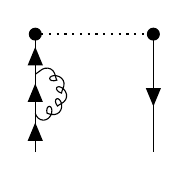
\begin{tikzpicture}[baseline=($(a)!0.5!(exa)$.base)]
			\begin{feynman}
				\node[dot] (a);
				\node[right=\FDWidth of a,dot] (b);
				\vertex[below=\FDHeight of a] (exa);
				\vertex[below=\FDHeight of b] (exb);
				\vertex at ($(exa)!0.33!(a)$) (a1);
				\vertex at ($(exa)!0.66!(a)$) (a2);
				\diagram*{
				(a) --[ghost] (b);
				(exa) --[fermion] (a1) --[fermion] (a2) --[fermion] (a);
				(b) --[fermion] (exb);
				(a1) --[gluon, half right,looseness=2] (a2);
				};
			\end{feynman}
		\end{tikzpicture}
	}\hfil
	\subfloat[]{
		\centering
		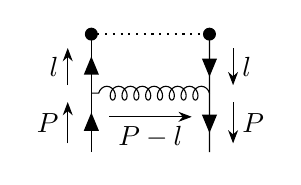
\begin{tikzpicture}[baseline=($(a)!0.5!(exa)$.base)]
			\begin{feynman}
				\node[dot] (a);
				\node[right=\FDWidth of a,dot] (b);
				\vertex[below=\FDHeight of a] (exa);
				\vertex[below=\FDHeight of b] (exb);
				\vertex at ($(exa)!0.5!(a)$) (a1);
				\vertex at ($(exb)!0.5!(b)$) (b1);
				\diagram*{
				(a) --[ghost] (b);
				(exa) --[fermion,momentum=\(P\)] (a1) --[fermion,momentum=\(l\)] (a);
				(b) --[fermion,momentum=\(l\)] (b1) --[fermion,momentum=\(P\)] (exb);
				(b1) --[gluon,rmomentum=\(P-l\)] (a1);
				};
			\end{feynman}
		\end{tikzpicture}
		\label{1b}
	}\hfil
	\caption{}
\end{figure}

The Feynman rule for the composite operator is
\begin{align}
	\feynmandiagram[small,baseline=(a.base),horizontal=a to b]{
	a[dot, label={\(p_1\),0}] --[ghost] b[dot, label={\(p_2\),z}];
	};=e^{-ip_2^zz} \gamma^z
\end{align}
and two external lines give $\bar u(P)$ and $u(P)$ respectively.

The first one is a quark self-energy correction
\begin{align}
	\bar u(P)e^{-iP^zz} \gamma^z \frac{i(\slashed{P}+m)}{P^2-m^2}\pqty{-i\Sigma_2(P)} u(P)
\end{align}
% where $\Sigma_2$ follows Peskin's result\cite{MichaelE.Peskin1995}. 

The second one is
\begin{align}
	  & \bar u(P)\int\mmd[1]{l^0}\mmd[2]{\vb{l}_T}\eval{(-ig_st^a\gamma^{\mu})\frac{i(\slashed{l}+m)}{l^2-m^2}\gamma^z\frac{i(\slashed{l}+m)}{l^2-m^2}(-ig_st^a\gamma^{\nu})\tilde D_{G\mu\nu}^A(P-l)u(P)}_{l^z=xP^z}\notag \\
	  & =-g_s^2C_F\bar u(P)\int\mmd[1]{l^0}\mmd[2]{\vb{l}_T}\eval{\gamma^{\mu}\frac{i(\slashed{l}+m)}{l^2-m^2}\gamma^z\frac{i(\slashed{l}+m)}{l^2-m^2}\gamma^{\nu}\tilde D_{G\mu\nu}^A(P-l)u(P)}_{l^z=xP^z}
\end{align}
For the definition of $\tilde D_{G\mu\nu}^A$, see Section~\ref{sec:conv}. There're in total 6 poles:
\begin{center}
	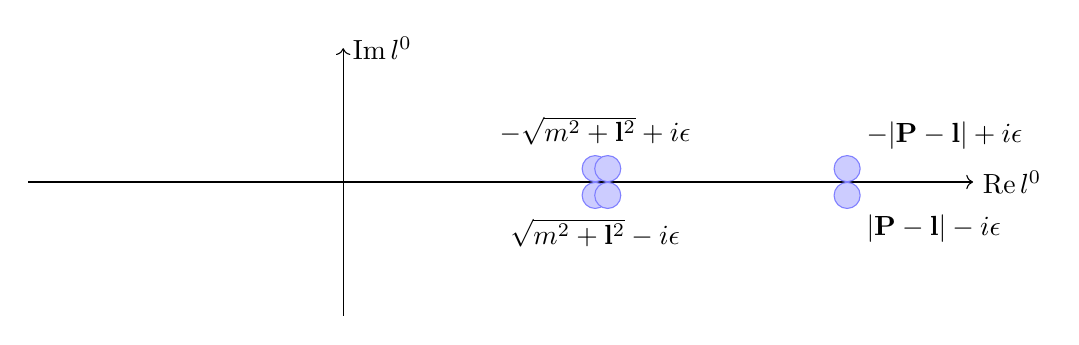
\begin{tikzpicture}[xscale=8,yscale=1.7]
		\draw[->] (-.5,0) -- (1,0) node[right]{$\Re l^0$};
		\draw[->] (0,-1) -- (0,1) node[right]{$\Im l^0$};
		\node at (.8,.1) [circle,draw=blue!50,fill=blue!20,label=above right:{$-\abs{\vb{P}-\vb{l}}+i\epsilon$}] {};
		\node at (.8,-.1) [circle,draw=blue!50,fill=blue!20,label=below right:{$\abs{\vb{P}-\vb{l}}-i\epsilon$}] {};
		\node at (0.4,.1) [circle,draw=blue!50,fill=blue!20,label=above:{$-\sqrt{m^2+\vb{l}^2}+i\epsilon$}] {};
		\node at (0.4,-.1) [circle,draw=blue!50,fill=blue!20,label=below:{$\sqrt{m^2+\vb{l}^2}-i\epsilon$}] {};
		\node at (0.42,.1) [circle,draw=blue!50,fill=blue!20] {};
		\node at (0.42,-.1) [circle,draw=blue!50,fill=blue!20] {};
	\end{tikzpicture}
\end{center}
For the result of numerator simplification, see Section~\ref{sec:dc1}
% The numerator is simplified as:
% \begin{align}
% 	&\bar u(P)\gamma^{\mu}(\slashed{P}-\slashed{l}+m)\gamma^z(\slashed{P}-\slashed{l}+m)\gamma^{\nu}u(P)\notag\\
% 	=&\left(2 l\cdot P-l^2-P^2+m^2\right) \bar u(P)\gamma^{\mu }\gamma^z\gamma^{\nu }u(P)+2 \left(l^z-P^z\right) \bar u(P)\gamma^{\mu }\slashed{l}\gamma^{\nu }u(P)\notag\\&-2 P^{\mu } \left(\bar u(P)\gamma^z\slashed{l}\gamma^{\nu }u(P)+\bar u(P)\slashed{l}\gamma^z\gamma^{\nu }u(P)-2	P^z \bar u(P)\gamma^{\nu }u(P)\right)
% \end{align}
% Adding the numerator of the axial gauge gluon propagator, the final result is 
% \begin{align}
% 	\frac{2 l^4 P^3}{\left(l^3\right)^2}+\frac{16 l^2 \left(P^3\right)^2}{l^3}-\frac{8 l^2 l^0P^0 P^3}{\left(l^3\right)^2}+4 l^2 P^3-\frac{4 l^2 l^0 P^0}{l^3}-8 m^2l^3+16 l^3 \left(P^3\right)^2-\frac{32 l^0 P^0 \left(P^3\right)^2}{l^3}\notag\\-8l^0 l^3 P^0+8 \left(l^3\right)^2 P^3-24 l^0 P^0 P^3+\frac{8\left(l^0\right)^2 \left(P^0\right)^2 P^3}{\left(l^3\right)^2}+\frac{8 \left(l^0\right)^2\left(P^0\right)^2}{l^3}+8 m^2 P^3+24 \left(P^3\right)^3
% \end{align}

\section{One Loop Quasi PDF (Feynman Gauge)}
In Feynman gauge, we must have the full definition of quasi PDF. For unpolarized quasi PDF
\begin{align}
	\tilde{q}(x)=\frac{1}{2} \int \frac{\dd z}{2 \pi} e^{i x P^{z} z}\langle P, S|\bar{\psi}(z) \gamma^z \mathcal{P} \exp \left[i g \int_{0}^{z} \dd z^{\prime} A^{a,z}\left(z^{\prime}\right) \mathrm{t}^{a}\right] \psi(0)| P, S\rangle
\end{align}
There're following 8 diagrams.
\def\FDWidth{3cm}
\def\FDHeight{3cm}
\begin{figure}[!htpb]
	\centering
	\hfil\subfloat[]{
		\centering
		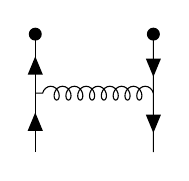
\begin{tikzpicture}[baseline=($(a)!0.5!(exa)$.base)]
			\begin{feynman}
				\node[dot] (a);
				\node[right=\FDWidth of a,dot] (b);
				\vertex[below=\FDHeight of a] (exa);
				\vertex[below=\FDHeight of b] (exb);
				\vertex at ($(exa)!0.5!(a)$) (a1);
				\vertex at ($(exb)!0.5!(b)$) (b1);
				\diagram*{
				% (a) --[Eikonal] (b);
				(exa) --[fermion] (a1) --[fermion] (a);
				(b) --[fermion] (b1) --[fermion] (exb);
				(b1) --[gluon] (a1);
				};
			\end{feynman}
		\end{tikzpicture}
		\label{2:nogl}
	}\hfil
	\subfloat[]{
		\centering
		\begin{tikzpicture}[baseline=($(a)!0.5!(exa)$.base)]
			\begin{feynman}
				\node[dot] (a);
				\node[right=\FDWidth of a,dot] (b);
				\vertex at ($(a)!0.5!(b)$) (o);
				\vertex[below=\FDHeight of a] (exa);
				\vertex[below=\FDHeight of b] (exb);
				\vertex at ($(exa)!0.5!(a)$) (a1);
				\vertex at ($(exb)!0.5!(b)$) (b1);
				\diagram*{
				(o) --[Eikonal] (b);
				(exa) --[fermion] (a1) --[fermion] (a);
				(b) --[fermion] (exb);
				(a1) --[gluon] (o);
				};
			\end{feynman}
		\end{tikzpicture}
		\label{2/-}
	}\hfil
	\subfloat[]{
		\centering
		\begin{tikzpicture}[baseline=($(a)!0.5!(exa)$.base)]
			\begin{feynman}
				\node[dot] (a);
				\node[right=\FDWidth of a,dot] (b);
				\vertex at ($(a)!0.5!(b)$) (o);
				\vertex[below=\FDHeight of a] (exa);
				\vertex[below=\FDHeight of b] (exb);
				\vertex at ($(exa)!0.5!(a)$) (a1);
				\vertex at ($(exb)!0.5!(b)$) (b1);
				\diagram*{
				(a) --[Eikonal] (o);
				(exa) --[fermion] (a);
				(b) --[fermion] (b1) --[fermion] (exb);
				(b1) --[gluon] (o);
				};
			\end{feynman}
		\end{tikzpicture}
		\label{2-`}
	}\hfil
	\subfloat[]{
		\centering
		\begin{tikzpicture}[baseline=($(a)!0.5!(exa)$.base)]
			\begin{feynman}
				\node[dot] (a);
				\node[right=\FDWidth of a,dot] (b);
				\vertex at ($(a)!0.3!(b)$) (o1);
				\vertex at ($(a)!0.7!(b)$) (o2);
				\vertex[below=\FDHeight of a] (exa);
				\vertex[below=\FDHeight of b] (exb);
				\diagram*{
				(a) --[Eikonal] (o1);
				(b) --[Eikonal] (o2);
				(exa) --[fermion] (a);
				(b) --[fermion] (exb);
				(o1) --[gluon, half right] (o2);
				};
			\end{feynman}
		\end{tikzpicture}
		\label{2-v-}
	}\hfil\\\hfil
	\subfloat[]{
		\centering
		\begin{tikzpicture}[baseline=($(a)!0.5!(exa)$.base)]
			\begin{feynman}
				\node[dot] (a);
				\node[right=\FDWidth of a,dot] (b);
				\vertex at ($(a)!0.5!(b)$) (o);
				\vertex[below=\FDHeight of a] (exa);
				\vertex[below=\FDHeight of b] (exb);
				\vertex at ($(exa)!0.5!(a)$) (a1);
				\vertex at ($(exb)!0.5!(b)$) (b1);
				\diagram*{
				(o) --[Eikonal] (a);
				(exa) --[fermion] (a1) --[fermion] (a);
				(b) --[fermion] (exb);
				(a1) --[gluon] (o);
				};
			\end{feynman}
		\end{tikzpicture}
		\label{2-/}
	}\hfil
	\subfloat[]{
		\centering
		\begin{tikzpicture}[baseline=($(a)!0.5!(exa)$.base)]
			\begin{feynman}
				\node[dot] (a);
				\node[right=\FDWidth of a,dot] (b);
				\vertex at ($(a)!0.5!(b)$) (o);
				\vertex[below=\FDHeight of a] (exa);
				\vertex[below=\FDHeight of b] (exb);
				\vertex at ($(exa)!0.5!(a)$) (a1);
				\vertex at ($(exb)!0.5!(b)$) (b1);
				\diagram*{
				(b) --[Eikonal] (o);
				(exa) --[fermion] (a);
				(b) --[fermion] (b1) --[fermion] (exb);
				(b1) --[gluon] (o);
				};
			\end{feynman}
		\end{tikzpicture}
		\label{2`-}
	}\hfil
	\subfloat[]{
		\centering
		\begin{tikzpicture}[baseline=($(a)!0.5!(exa)$.base)]
			\begin{feynman}
				\node[dot] (a);
				\node[right=\FDWidth of a,dot] (b);
				\vertex at ($(a)!0.5!(b)$) (o);
				\vertex at ($(a)!0.2!(b)$) (o1);
				\vertex at ($(a)!0.8!(b)$) (o2);
				\vertex[below=\FDHeight of a] (exa);
				\vertex[below=\FDHeight of b] (exb);
				\diagram*{
				(a) --[Eikonal] (o);
				(exa) --[fermion] (a);
				(b) --[fermion] (exb);
				(o1) --[gluon, half right] (o);
				};
			\end{feynman}
		\end{tikzpicture}
		\label{2-o}
	}\hfil
	\subfloat[]{
		\centering
		\begin{tikzpicture}[baseline=($(a)!0.5!(exa)$.base)]
			\begin{feynman}
				\node[dot] (a);
				\node[right=\FDWidth of a,dot] (b);
				\vertex at ($(a)!0.5!(b)$) (o);
				\vertex at ($(a)!0.2!(b)$) (o1);
				\vertex at ($(a)!0.8!(b)$) (o2);
				\vertex[below=\FDHeight of a] (exa);
				\vertex[below=\FDHeight of b] (exb);
				\diagram*{
				(b) --[Eikonal] (o);
				(exa) --[fermion] (a);
				(b) --[fermion] (exb);
				(o) --[gluon, half right] (o2);
				};
			\end{feynman}
		\end{tikzpicture}
		\label{2o-}
	}\hfil\\\hfil
	\subfloat[]{
		\centering
		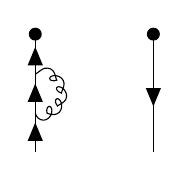
\begin{tikzpicture}[baseline=($(a)!0.5!(exa)$.base)]
			\begin{feynman}
				\node[dot] (a);
				\node[right=\FDWidth of a,dot] (b);
				\vertex[below=\FDHeight of a] (exa);
				\vertex[below=\FDHeight of b] (exb);
				\vertex at ($(exa)!0.33!(a)$) (a1);
				\vertex at ($(exa)!0.66!(a)$) (a2);
				\diagram*{
				% (a) --[Eikonal] (b);
				(exa) --[fermion] (a1) --[fermion] (a2) --[fermion] (a);
				(b) --[fermion] (exb);
				(a1) --[gluon, half right,looseness=2] (a2);
				};
			\end{feynman}
		\end{tikzpicture}
	}\hfil
	\subfloat[]{
		\centering
		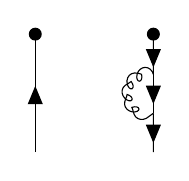
\begin{tikzpicture}[baseline=($(a)!0.5!(exa)$.base)]
			\begin{feynman}
				\node[dot] (a);
				\node[right=\FDWidth of a,dot] (b);
				\vertex[below=\FDHeight of a] (exa);
				\vertex[below=\FDHeight of b] (exb);
				\vertex at ($(exb)!0.33!(b)$) (b1);
				\vertex at ($(exb)!0.66!(b)$) (b2);
				\diagram*{
				% (a) --[Eikonal] (b);
				(exa) --[fermion] (a);
				(b) --[fermion] (b2) --[fermion] (b1) --[fermion] (exb);
				(b2) --[gluon, half right,looseness=2] (b1);
				};
			\end{feynman}
		\end{tikzpicture}
	}\hfil
	\caption{Diagrams of quasi PDF in Feynman gauge. }
\end{figure}

The corresponding Feynman rules are:
\begin{align}
	\feynmandiagram[small, horizontal=a to g,baseline=(a.base), layered layout]{
	a --[Eikonal,momentum=\(k\)] b --[gluon, momentum=\(k\)] g;
	};=-ig_st^an^{\mu};\qquad              & \int \qquad
	\feynmandiagram[small, horizontal=g to a,baseline=(a.base), layered layout]{
	a --[Eikonal,momentum'=\(k\)] b --[gluon, momentum'=\(k\)] g;
	};=ig_st^an^{\mu};\\
	\feynmandiagram[small, horizontal=a to c,baseline=(b.base), layered layout]{
	a --[Eikonal] b --[Eikonal] c;
	b --[gluon] g;
	};=-ig_st^an^{\mu};\qquad              & \int \qquad
	\feynmandiagram[small, horizontal=a to c,baseline=(b.base), layered layout]{
	a --[Eikonal] b --[Eikonal] c;
	b --[gluon] g;
	};=ig_st^an^{\mu};\\
	\feynmandiagram[small, horizontal=a to b,baseline=(a.base)]{
	a[dot] --[Eikonal,momentum=\(k\)] b;
	};=\frac{i}{n\cdot k+i\epsilon};\qquad & \int \qquad
	\feynmandiagram[small, horizontal=a to b,baseline=(a.base)]{
	a --[Eikonal,rmomentum=\(k\)] b[dot];
	};=\frac{i}{n\cdot k+i\epsilon};\\
	\feynmandiagram[small, horizontal=a to b,baseline=(a.base)]{
	a --[fermion,momentum=\(k\)] b[dot];
	};\qquad                               & \int \qquad
	\feynmandiagram[small, horizontal=a to b,baseline=(a.base)]{
	a[dot] --[fermion,momentum=\(k\)] b;
	};
\end{align}
The last line stands for the momentum conservation between two dots. There're also an extra $1/2$ factor on the outside and a Dirac delta function to eliminate all $z$-direction loop momenta. The delta function confines the sum of all momenta flow in $z$ equals to $xP^z$.

Let's take the spin sum of external states.

\def\FDWidthS{2cm}
\def\FDHeightS{2cm}
\subsection{Real corrections}
First we must deal with those real diagrams.

Diagram~\ref{2:nogl} gives
\begin{align}
	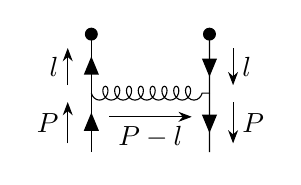
\begin{tikzpicture}[baseline=($(a)!0.5!(exa)$.base)]
		\begin{feynman}
			\node[dot] (a);
			\node[right=\FDWidthS of a,dot] (b);
			\vertex[below=\FDHeightS of a] (exa);
			\vertex[below=\FDHeightS of b] (exb);
			\vertex at ($(exa)!0.5!(a)$) (a1);
			\vertex at ($(exb)!0.5!(b)$) (b1);
			\diagram*{
			% (a) --[Eikonal] (b);
			(exa) --[fermion,momentum=\(P\)] (a1) --[fermion,momentum=\(l\)] (a);
			(b) --[fermion,momentum=\(l\)] (b1) --[fermion,momentum=\(P\)] (exb);
			(a1) --[gluon,momentum'=\(P-l\)] (b1);
			};
		\end{feynman}
	\end{tikzpicture} & =\frac{1}{2}\bar u(P) \pqty{-ig_st^a\gamma_\nu} \int\mm{l}\frac{i}{\slashed l-m+i\epsilon}\gamma^z\frac{-ig^{\mu \nu}}{(P-l)^2+i\epsilon} \frac{i}{\slashed l-m+i\epsilon}\pqty{-ig_s\gamma_{\mu}t^a}u(P)\delta(l^z-xP^z)\notag \\
	                            & =-i\frac{g_s^2C_F}{2}\int\mm{l}\bar u(P) \gamma^\mu \frac{\slashed l+m}{l^2-m^2+i\epsilon}\gamma^z\frac{\slashed l+m}{l^2-m^2+i\epsilon}\gamma_{\mu} u(P)\frac{1}{(P-l)^2+i\epsilon}\delta(l^z-xP^z)
\end{align}
After spin sum:
\begin{align}
	\frac{1}{2}\sum_s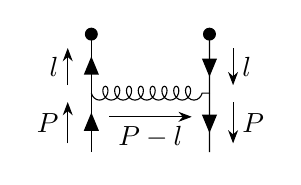
\begin{tikzpicture}[baseline=($(a)!0.5!(exa)$.base)]
		\begin{feynman}
			\node[dot] (a);
			\node[right=\FDWidthS of a,dot] (b);
			\vertex[below=\FDHeightS of a] (exa);
			\vertex[below=\FDHeightS of b] (exb);
			\vertex at ($(exa)!0.5!(a)$) (a1);
			\vertex at ($(exb)!0.5!(b)$) (b1);
			\diagram*{
			% (a) --[Eikonal] (b);
			(exa) --[fermion,momentum=\(P\)] (a1) --[fermion,momentum=\(l\)] (a);
			(b) --[fermion,momentum=\(l\)] (b1) --[fermion,momentum=\(P\)] (exb);
			(a1) --[gluon,momentum'=\(P-l\)] (b1);
			};
		\end{feynman}
	\end{tikzpicture} & =\frac{-ig_s^2C_F}{4}\int\mm{l}\sum_s\bar u(P) \gamma^\mu \frac{\slashed l+m}{l^2-m^2+i\epsilon}\gamma^z\frac{\slashed l+m}{l^2-m^2+i\epsilon}\gamma_{\mu} u(P)\frac{1}{(P-l)^2+i\epsilon}\delta(l^z-xP^z)\notag \\
	                                             & =\frac{-ig_s^2C_F}{4}\int\mm{l} \frac{\Tr{(\slashed P+m)\gamma^\mu(\slashed l+m)\gamma^z(\slashed l+m)\gamma_{\mu}}}{(l^2-m^2+i\epsilon)^2(P-l)^2}\delta(l^z-xP^z)\notag                                         \\
	\intertext{the numerator and the denominator of the integrand is checked out in this step with Xiong's result}
	                                             & =
\end{align}
Diagram~\ref{2/-} gives
\begin{align}
	\begin{tikzpicture}[baseline=($(a)!0.5!(exa)$.base)]
		\begin{feynman}
			\node[dot] (a);
			\node[right=\FDWidthS of a,dot] (b);
			\vertex at ($(a)!0.5!(b)$) (o);
			\vertex[below=\FDHeightS of a] (exa);
			\vertex[below=\FDHeightS of b] (exb);
			\vertex at ($(exa)!0.5!(a)$) (a1);
			\vertex at ($(exb)!0.5!(b)$) (b1);
			\diagram*{
			(o) --[Eikonal,momentum=\(P-l\)] (b);
			(exa) --[fermion,momentum=\(P\)] (a1) --[fermion,momentum=\(l\)] (a);
			(b) --[fermion,momentum=\(P\)] (exb);
			(a1) --[gluon,momentum'=\(P-l\)] (o);
			};
		\end{feynman}
	\end{tikzpicture} & =\frac{1}{2}\bar u(P) \gamma^z \int\mm{l}\frac{i}{l^z-P^z+i\epsilon}\pqty{ig_st^a}\frac{-ig^{\mu z}}{(P-l)^2+i\epsilon} \frac{i}{\slashed l-m+i\epsilon}\pqty{-ig_s\gamma_{\mu}t^a}u(P)\delta(l^z-xP^z)\notag \\
	                            & =\frac{ig_s^2C_F}{2}\int\mm{l}\bar u(P) \gamma^z \frac{\slashed l+m}{l^2-m^2+i\epsilon}\gamma^zu(P)\frac{1}{l^z-P^z+i\epsilon}\frac{1}{(P-l)^2+i\epsilon} \delta(l^z-xP^z)
\end{align}
Take the spin sum
\begin{align}
	\frac{1}{2}\sum_s\begin{tikzpicture}[baseline=($(a)!0.5!(exa)$.base)]
		\begin{feynman}
			\node[dot] (a);
			\node[right=\FDWidthS of a,dot] (b);
			\vertex at ($(a)!0.5!(b)$) (o);
			\vertex[below=\FDHeightS of a] (exa);
			\vertex[below=\FDHeightS of b] (exb);
			\vertex at ($(exa)!0.5!(a)$) (a1);
			\vertex at ($(exb)!0.5!(b)$) (b1);
			\diagram*{
			(o) --[Eikonal,momentum=\(P-l\)] (b);
			(exa) --[fermion,momentum=\(P\)] (a1) --[fermion,momentum=\(l\)] (a);
			(b) --[fermion,momentum=\(P\)] (exb);
			(a1) --[gluon,momentum'=\(P-l\)] (o);
			};
		\end{feynman}
	\end{tikzpicture} & =\sum_s\frac{ig_s^2C_F}{4}\int\mm{l}\bar u(P) \gamma^z \frac{\slashed l+m}{l^2-m^2+i\epsilon}\gamma^zu(P)\frac{1}{l^z-P^z+i\epsilon}\frac{1}{(P-l)^2+i\epsilon} \delta(l^z-xP^z)\notag   \\
	                                             & =\frac{ig_s^2C_F}{4}\int\mm{l}  \frac{\Tr{(\slashed P+m)\gamma^z(\slashed l+m)\gamma^z}}{l^2-m^2+i\epsilon}\frac{1}{l^z-P^z+i\epsilon}\frac{1}{(P-l)^2+i\epsilon} \delta(l^z-xP^z)\notag \\
\end{align}
Diagram~\ref{2-`} should be the same with Diagram~\ref{2/-}.
\begin{align}
	\begin{tikzpicture}[baseline=($(a)!0.5!(exa)$.base)]
		\begin{feynman}
			\node[dot] (a);
			\node[right=\FDWidthS of a,dot] (b);
			\vertex at ($(a)!0.5!(b)$) (o);
			\vertex[below=\FDHeightS of a] (exa);
			\vertex[below=\FDHeightS of b] (exb);
			\vertex at ($(exa)!0.5!(a)$) (a1);
			\vertex at ($(exb)!0.5!(b)$) (b1);
			\diagram*{
			(a) --[Eikonal,momentum=\(P-l\)] (o);
			(exa) --[fermion,momentum=\(P\)] (a);
			(b) --[fermion,momentum=\(l\)] (b1) --[fermion,momentum=\(P\)] (exb);
			(o) --[gluon,momentum'=\(P-l\)] (b1);
			};
		\end{feynman}
	\end{tikzpicture} & =\frac{1}{2}\bar u(P) \pqty{-ig_s\gamma_{\mu}t^a}\int\mm{l}\frac{i}{\slashed l-m+i\epsilon}\frac{-ig^{\mu z}}{(P-l)^2+i\epsilon} \frac{i}{P^z-l^z+i\epsilon}\pqty{-ig_st^a}\gamma^z u(P)\delta(l^z-xP^z)\notag \\
	                            & =\frac{ig_s^2C_F}{2}\int\mm{l}\bar u(P) \gamma^z \frac{\slashed l+m}{l^2-m^2+i\epsilon}\gamma^zu(P)\frac{1}{l^z-P^z+i\epsilon}\frac{1}{(P-l)^2+i\epsilon} \delta(l^z-xP^z)
\end{align}

Diagram~\ref{2-v-} is
\begin{align}
	\begin{tikzpicture}[baseline=($(a)!0.5!(exa)$.base)]
		\begin{feynman}
			\node[dot] (a);
			\node[right=\FDWidthS of a,dot] (b);
			\vertex at ($(a)!0.3!(b)$) (o1);
			\vertex at ($(a)!0.7!(b)$) (o2);
			\vertex[below=\FDHeightS of a] (exa);
			\vertex[below=\FDHeightS of b] (exb);
			\diagram*{
			(a) --[Eikonal,momentum=\(l\)] (o1);
			(b) --[Eikonal,rmomentum'=\(l\)] (o2);
			(exa) --[fermion,momentum=\(P\)] (a);
			(b) --[fermion,momentum=\(P\)] (exb);
			(o1) --[gluon, half right,momentum'=\(l\)] (o2);
			};
		\end{feynman}
	\end{tikzpicture} & =\frac{1}{2}\bar u(P)\gamma^z\int\mm{l}\frac{i}{l^z+i\epsilon}\pqty{ig_st^a}\frac{-ig^{zz}}{l^2+i\epsilon}\pqty{-ig_st^a}\frac{i}{-l^z+i\epsilon} u(P)\delta(l^z-(1-x)P^z)\notag \\
	                            & =\frac{-ig_s^2C_F}{2}\int\mm{l}\bar u(P)\gamma^zu(P)\frac{1}{l^z+i\epsilon}\frac{1}{l^2+i\epsilon}\frac{1}{-l^z+i\epsilon} \delta(l^z-(1-x)P^z)
\end{align}
Take the spin sum
\begin{align}
	\frac{1}{2}\sum_s\begin{tikzpicture}[baseline=($(a)!0.5!(exa)$.base)]
		\begin{feynman}
			\node[dot] (a);
			\node[right=\FDWidthS of a,dot] (b);
			\vertex at ($(a)!0.3!(b)$) (o1);
			\vertex at ($(a)!0.7!(b)$) (o2);
			\vertex[below=\FDHeightS of a] (exa);
			\vertex[below=\FDHeightS of b] (exb);
			\diagram*{
			(a) --[Eikonal,momentum=\(l\)] (o1);
			(b) --[Eikonal,rmomentum'=\(l\)] (o2);
			(exa) --[fermion,momentum=\(P\)] (a);
			(b) --[fermion,momentum=\(P\)] (exb);
			(o1) --[gluon, half right,momentum'=\(l\)] (o2);
			};
		\end{feynman}
	\end{tikzpicture}
	  & =\sum_s\frac{-ig_s^2C_F}{4}\int\mm{l}\bar u(P)\gamma^zu(P)\frac{1}{l^z+i\epsilon}\frac{1}{l^2+i\epsilon}\frac{1}{-l^z+i\epsilon} \delta(l^z-(1-x)P^z)\notag \\
	  & =\frac{-ig_s^2C_F}{4}\int\mm{l}\Tr{(\slashed P+m)\gamma^z}\frac{1}{l^z+i\epsilon}\frac{1}{l^2+i\epsilon}\frac{1}{-l^z+i\epsilon} \delta(l^z-(1-x)P^z)
\end{align}

\subsection{Virtual corrections}
The quark self energy diagram gives
\begin{align}
	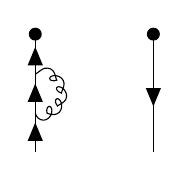
\begin{tikzpicture}[baseline=($(a)!0.5!(exa)$.base)]
		\begin{feynman}
			\node[dot] (a);
			\node[right=\FDWidthS of a,dot] (b);
			\vertex[below=\FDHeightS of a] (exa);
			\vertex[below=\FDHeightS of b] (exb);
			\vertex at ($(exa)!0.33!(a)$) (a1);
			\vertex at ($(exa)!0.66!(a)$) (a2);
			\diagram*{
			% (a) --[Eikonal] (b);
			(exa) --[fermion] (a1) --[fermion] (a2) --[fermion] (a);
			(b) --[fermion] (exb);
			(a1) --[gluon, half right,looseness=2] (a2);
			};
		\end{feynman}
	\end{tikzpicture}
\end{align}
and the divergence it brings should exactly cancel the divergence of all other diagrams since the operator is conserved current and all external legs are on-shell. With standard prescription, we perform a derivative operation on the self energy loop to extract the $Z_F$ factor. In the end we have $Z_F\delta(1-x)$.

Diagram~\ref{2-/} corresponds to the vertex correction of a heavy-light current for HQET
\begin{align}
	\begin{tikzpicture}[baseline=($(a)!0.5!(exa)$.base)]
		\begin{feynman}
			\node[dot] (a);
			\node[right=\FDWidthS of a,dot] (b);
			\vertex at ($(a)!0.5!(b)$) (o);
			\vertex[below=\FDHeightS of a] (exa);
			\vertex[below=\FDHeightS of b] (exb);
			\vertex at ($(exa)!0.5!(a)$) (a1);
			\vertex at ($(exb)!0.5!(b)$) (b1);
			\diagram*{
			(o) --[Eikonal,momentum'=\(P-l\)] (a);
			(exa) --[fermion,momentum=\(l\)] (a1) --[fermion,momentum=\(P\)] (a);
			(b) --[fermion,momentum=\(P\)] (exb);
			(a1) --[gluon,momentum'=\(P-l\)] (o);
			};
		\end{feynman}
	\end{tikzpicture} & =\frac{1}{2P^z}\bar u(P)\gamma^z\int\mm{l}\frac{i}{l^z-P^z+i\epsilon}(-ig_st^a)\frac{-ig^{\mu z}}{(P-l)^2+i\epsilon}\frac{i}{\slashed l-m+i\epsilon}(-ig_s\gamma_\mu)u(P)\delta(1-x)\notag \\
	                            & =\frac{-ig_s^2C_F}{2P^z}\int\mm{l}\bar u(P)\gamma^z\frac{\slashed l+m}{l^2-m^2+i\epsilon}\gamma^zu(P)\frac{1}{l^z-P^z+i\epsilon}\frac{1}{(P-l)^2+i\epsilon}\delta(1-x)
\end{align}
The other diagram \ref{2/-} is
\begin{align}
	\begin{tikzpicture}[baseline=($(a)!0.5!(exa)$.base)]
		\begin{feynman}
			\node[dot] (a);
			\node[right=\FDWidthS of a,dot] (b);
			\vertex at ($(a)!0.5!(b)$) (o);
			\vertex[below=\FDHeightS of a] (exa);
			\vertex[below=\FDHeightS of b] (exb);
			\vertex at ($(exa)!0.5!(a)$) (a1);
			\vertex at ($(exb)!0.5!(b)$) (b1);
			\diagram*{
			(o) --[Eikonal,momentum=\(P-l\)] (b);
			(exa) --[fermion,momentum=\(P\)] (a1) --[fermion,momentum=\(l\)] (a);
			(b) --[fermion,momentum=\(P\)] (exb);
			(a1) --[gluon,momentum'=\(P-l\)] (o);
			};
		\end{feynman}
	\end{tikzpicture}
	  & =\frac{ig_s^2C_F}{2}\int\mm{l}\bar u(P) \gamma^z \frac{\slashed l+m}{l^2-m^2+i\epsilon}\gamma^zu(P)\frac{1}{l^z-P^z+i\epsilon}\frac{1}{(P-l)^2+i\epsilon} \delta(l^z-xP^z)
\end{align}
The sum of both diagrams is
\begin{align}
	  & \begin{tikzpicture}[baseline=($(a)!0.5!(exa)$.base)]
		\begin{feynman}
			\node[dot] (a);
			\node[right=\FDWidthS of a,dot] (b);
			\vertex at ($(a)!0.5!(b)$) (o);
			\vertex[below=\FDHeightS of a] (exa);
			\vertex[below=\FDHeightS of b] (exb);
			\vertex at ($(exa)!0.5!(a)$) (a1);
			\vertex at ($(exb)!0.5!(b)$) (b1);
			\diagram*{
			(o) --[Eikonal,momentum=\(P-l\)] (b);
			(exa) --[fermion,momentum=\(P\)] (a1) --[fermion,momentum=\(l\)] (a);
			(b) --[fermion,momentum=\(P\)] (exb);
			(a1) --[gluon,momentum'=\(P-l\)] (o);
			};
		\end{feynman}
	\end{tikzpicture}+
	\begin{tikzpicture}[baseline=($(a)!0.5!(exa)$.base)]
		\begin{feynman}
			\node[dot] (a);
			\node[right=\FDWidthS of a,dot] (b);
			\vertex at ($(a)!0.5!(b)$) (o);
			\vertex[below=\FDHeightS of a] (exa);
			\vertex[below=\FDHeightS of b] (exb);
			\vertex at ($(exa)!0.5!(a)$) (a1);
			\vertex at ($(exb)!0.5!(b)$) (b1);
			\diagram*{
			(o) --[Eikonal,momentum'=\(P-l\)] (a);
			(exa) --[fermion,momentum=\(l\)] (a1) --[fermion,momentum=\(P\)] (a);
			(b) --[fermion,momentum=\(P\)] (exb);
			(a1) --[gluon,momentum'=\(P-l\)] (o);
			};
		\end{feynman}
	\end{tikzpicture}
	\notag\\
	  & =\frac{ig_s^2C_F}{2}\int\dd z\int\mm{l}\bar u(P) \gamma^z \frac{\slashed l+m}{l^2-m^2+i\epsilon}\gamma^zu(P)\frac{1}{l^z-P^z+i\epsilon}\frac{1}{(P-l)^2+i\epsilon} \bqty{e^{i(l^z-xP^z)z}-e^{i(P^z-xP^z)z}} \\
	  & =\frac{ig_s^2C_F}{2}\int\mm{l}\bar u(P) \gamma^z \frac{\slashed l+m}{l^2-m^2+i\epsilon}\gamma^zu(P)\frac{1}{l^z-P^z+i\epsilon}\frac{1}{(P-l)^2+i\epsilon} \bqty{\delta(l^z-xP^z)-\delta(P^z-xP^z)}
\end{align}
Here we're to take the spin sum. After integrated out $l^0$ and $\vb{l}_T$, the remaining integrand is \endnote{The constant mentioned above is
	\begin{align*}
		  & -\frac{C_F g_s^2 \left(-\sqrt{\left(m^2+P_3^2\right) \left(\Lambda ^2+m^2+P_3^2\right)}-\frac{2 P_3^2 \left(\log  \left(2 \left(m^2+P_3^2\right)\right)\right)}{\sqrt{\left(m^2+P_3^2\right) \left(\Lambda ^2+m^2+P_3^2\right)}+m^2+P_3^2}+\Lambda  \sqrt{m^2+P_3^2}+m^2+P_3^2\right)}{16 \pi ^2 \left(P_3-l_3\right) \sqrt{m^2+P_3^2}}-\frac{C_F g_s^2}{16 \pi ^2 \text{sgn}\left(l_3-P_3\right)}                                                                       \\
		  & \frac{P_3 C_F g_s^2 \left(\log  \left(l_3-P_3\right){}^2-\frac{2 \left(\log  \left(2 \left(\sqrt{\left(m^2+P_3^2\right) \left(\Lambda ^2+m^2+P_3^2\right)}-m^2-P_3^2\right)\right)\right)}{\Lambda }\right)}{16 \pi ^2 \sqrt{m^2+P_3^2}}+\frac{m^4 P_3 C_F g_s^2 \left(\Lambda -\Lambda  \sqrt{\frac{m^2+P_3^2}{\Lambda ^2+m^2+P_3^2}}\right)}{16 \pi ^2 \Lambda  \left(m^2+P_3^2\right){}^{3/2} \left(\Lambda ^2+m^2+P_3^2\right)}                                      \\
		  & -\frac{m^2 P_3^3 C_F g_s^2 \left(\Lambda  \sqrt{\frac{m^2+P_3^2}{\Lambda ^2+m^2+P_3^2}}+\sqrt{m^2+P_3^2}\right)}{8 \pi ^2 \Lambda  \left(m^2+P_3^2\right){}^{3/2} \left(\Lambda ^2+m^2+P_3^2\right)}-\frac{P_3^5 C_F g_s^2 \left(\Lambda +\Lambda  \sqrt{\frac{m^2+P_3^2}{\Lambda ^2+m^2+P_3^2}}+2 \sqrt{m^2+P_3^2}\right)}{16 \pi ^2 \Lambda  \left(m^2+P_3^2\right){}^{3/2} \left(\Lambda ^2+m^2+P_3^2\right)}                                                         \\
		  & -\frac{\Lambda ^2 m^2 P_3 C_F g_s^2 \left(\sqrt{\frac{m^2+P_3^2}{\Lambda ^2+m^2+P_3^2}}-1\right)}{16 \pi ^2 \left(m^2+P_3^2\right){}^{3/2} \left(\Lambda ^2+m^2+P_3^2\right)}-\frac{P_3^3 C_F g_s^2 \left(\Lambda  \left(\Lambda +\Lambda  \sqrt{\frac{m^2+P_3^2}{\Lambda ^2+m^2+P_3^2}}+2 \sqrt{m^2+P_3^2}\right)-2 \sqrt{\left(m^2+P_3^2\right) \left(\Lambda ^2+m^2+P_3^2\right)}\right)}{16 \pi ^2 \left(m^2+P_3^2\right){}^{3/2} \left(\Lambda ^2+m^2+P_3^2\right)}
	\end{align*}
	multiplied by the delta function and integration. }
\begin{align}
	  & \frac{g_s^2C_F{P^z}^3}{8\pi^2(m^2+{P^z}^2)}\int\dd l^z \frac{\delta(l^z-xP^z)-\delta(P^z-xP^z)}{{\abs{l^z-P^z}}}+\frac{g_s^2C_F{P^z}^2}{8\pi^2\sqrt{m^2+{P^z}^2}}\int\dd l^z \pqty{\frac{\log\frac{l^z-P^z}{\Lambda}}{{l^z-P^z}}}\bqty{\delta(l^z-xP^z)-\delta(P^z-xP^z)}+\text{Constant}\notag \\
	\intertext{by setting $l^z=yP^z$, $\dd l^z (\delta(l^z-xP^z)-\delta(P^z-xP^z))=\dd y (\delta(y-x)-\delta(1-x))$}
	  & =\frac{g_s^2C_F{P^z}^3/\abs{P^z}}{8\pi^2(m^2+{P^z}^2)}\int\dd y \frac{\delta(y-x)-\delta(1-x)}{{\abs{y-1}}}+\frac{g_s^2C_F{P^z}}{8\pi^2\sqrt{m^2+{P^z}^2}}\int\dd y \pqty{\frac{\log\frac{y-1}{\Lambda/P^z}}{{y-1}}}\bqty{\delta(y-x)-\delta(1-x)}+\text{Constant}\notag
\end{align}
Now we can transform the integration on $y$ to plus functions\endnote{Wrong prescription: Having $\pqty{\int_{0}^{\infty}-\int_1^{\infty}}\dd xF(x)\bqty{G(x)-G(1)}=\int_0^1\dd xF_+(x)G(x)$
	\begin{align}
		\int\dd y \frac{\delta(y-x)-\delta(1-x)}{{\abs{y-1}}}=\frac{\theta(1-x)\theta(x)}{(1-x)_+}+\frac{ \theta(-x)}{2(x-1)}+\frac{3 \theta(x-1)}{2(x-1)}+\frac{\theta(1-x)\theta(x)}{x-1}
	\end{align}
	\begin{align}
		\int\dd y \pqty{\frac{\log\frac{y-1}{\Lambda/P^z}}{{y-1}}}\bqty{\delta(y-x)-\delta(1-x)}=\pqty{\frac{\log\frac{y-1}{\Lambda/P^z}}{{y-1}}}_+ +\frac{\log \left(\frac{x-1}{\Lambda /P^z}\right)\theta(x-1)}{x-1}+\frac{\log (1-x)\theta(1-x)}{x-1}
	\end{align}}.
By redefining the plus function to an extended version:
\begin{align}
	f_{\boxplus}(x)=f(x)-\delta(1-x)\int_{-\infty}^\infty\dd yf(y)
\end{align}
The full result is
\begin{align}
	\bqty{\frac{1}{2}\sum_s\begin{tikzpicture}[baseline=($(a)!0.5!(exa)$.base)]
			\begin{feynman}
				\node[dot] (a);
				\node[right=\FDWidthS of a,dot] (b);
				\vertex at ($(a)!0.5!(b)$) (o);
				\vertex[below=\FDHeightS of a] (exa);
				\vertex[below=\FDHeightS of b] (exb);
				\vertex at ($(exa)!0.5!(a)$) (a1);
				\vertex at ($(exb)!0.5!(b)$) (b1);
				\diagram*{
				(o) --[Eikonal,momentum=\(P-l\)] (b);
				(exa) --[fermion,momentum=\(P\)] (a1) --[fermion,momentum=\(l\)] (a);
				(b) --[fermion,momentum=\(P\)] (exb);
				(a1) --[gluon,momentum'=\(P-l\)] (o);
				};
			\end{feynman}
		\end{tikzpicture}}_{\boxplus}
\end{align}
Diagram~\ref{2`-} is
\begin{align}
	\begin{tikzpicture}[baseline=($(a)!0.5!(exa)$.base)]
		\begin{feynman}
			\node[dot] (a);
			\node[right=\FDWidthS of a,dot] (b);
			\vertex at ($(a)!0.5!(b)$) (o);
			\vertex[below=\FDHeightS of a] (exa);
			\vertex[below=\FDHeightS of b] (exb);
			\vertex at ($(exa)!0.5!(a)$) (a1);
			\vertex at ($(exb)!0.5!(b)$) (b1);
			\diagram*{
			(b) --[Eikonal,momentum'=\(P-l\)] (o);
			(exa) --[fermion,momentum=\(P\)] (a);
			(b) --[fermion,momentum=\(l\)] (b1) --[fermion,momentum=\(P\)] (exb);
			(b1) --[gluon,rmomentum=\(P-l\)] (o);
			};
		\end{feynman}
	\end{tikzpicture} & =\frac{1}{2P^z}\int\mm{l}\bar u(P)(-ig_s\gamma_{\mu}t^a)\frac{i(\slashed l+m)}{l^2-m^2+i\epsilon}\gamma^z\frac{-ig^{\mu z}}{(P-l)^2+i\epsilon}\frac{i}{P^z-l^z}(ig_st^a)u(P)\delta(1-x)\notag \\
	                            & =\frac{-ig_s^2C_F}{2P^z}\int\mm{l}\bar u(P)\gamma^z\frac{\slashed l+m}{l^2-m^2+i\epsilon}\gamma^zu(P)\frac{1}{l^z-P^z-i\epsilon}\frac{1}{(P-l)^2+i\epsilon}\delta(1-x)\notag              \\
	                            & =\begin{tikzpicture}[baseline=($(a)!0.5!(exa)$.base)]
		\begin{feynman}
			\node[dot] (a);
			\node[right=\FDWidthS of a,dot] (b);
			\vertex at ($(a)!0.5!(b)$) (o);
			\vertex[below=\FDHeightS of a] (exa);
			\vertex[below=\FDHeightS of b] (exb);
			\vertex at ($(exa)!0.5!(a)$) (a1);
			\vertex at ($(exb)!0.5!(b)$) (b1);
			\diagram*{
			(o) --[Eikonal,momentum'=\(P-l\)] (a);
			(exa) --[fermion,momentum=\(l\)] (a1) --[fermion,momentum=\(P\)] (a);
			(b) --[fermion,momentum=\(P\)] (exb);
			(a1) --[gluon,momentum'=\(P-l\)] (o);
			};
		\end{feynman}
	\end{tikzpicture}
\end{align}
After spin sum diagram~\ref{2-/}
\begin{align}
	\frac{1}{2}\sum_s\begin{tikzpicture}[baseline=($(a)!0.5!(exa)$.base)]
		\begin{feynman}
			\node[dot] (a);
			\node[right=\FDWidthS of a,dot] (b);
			\vertex at ($(a)!0.5!(b)$) (o);
			\vertex[below=\FDHeightS of a] (exa);
			\vertex[below=\FDHeightS of b] (exb);
			\vertex at ($(exa)!0.5!(a)$) (a1);
			\vertex at ($(exb)!0.5!(b)$) (b1);
			\diagram*{
			(o) --[Eikonal,momentum'=\(P-l\)] (a);
			(exa) --[fermion,momentum=\(l\)] (a1) --[fermion,momentum=\(P\)] (a);
			(b) --[fermion,momentum=\(P\)] (exb);
			(a1) --[gluon,momentum'=\(P-l\)] (o);
			};
		\end{feynman}
	\end{tikzpicture} & =\frac{-ig_s^2C_F}{4P^z}\delta(1-x)\int\mm{l}\frac{\Tr{(\slashed P+m)\gamma^z(\slashed l+m)\gamma^z}}{l^2-m^2+i\epsilon}\frac{1}{n\cdot (l-P)+i\epsilon}\frac{1}{(P-l)^2+i\epsilon}
\end{align}
First we apply Feynman parametrization to the normal propagators
\begin{align}
	\frac{1}{l^2-m^2+i\epsilon}\frac{1}{(P-l)^2+i\epsilon}=\int_0^1\dd y\frac{1}{\bqty{(l+P (y-1))^2-ym^2 -P^2 (y-1) y}^2}
\end{align}
According to identity
\begin{align}
	\frac{1}{a^rb^s}=2^s\frac{\Gamma(r+s)}{\Gamma(r)\Gamma(s)}\int_0^\infty\dd\lambda\frac{\lambda^{s-1}}{(a+2b\lambda)^{r+s}}
\end{align}
the whole denominator becomes
\begin{align}
	\frac{2\Gamma(3)}{\Gamma(2)\Gamma(1)}\int_0^1\dd y\int_0^\infty\dd\lambda\frac{1}{\bqty{(l+\lambda  n+P (y-1))^2-ym^2 -\lambda ^2 n^2-2 \lambda  n P y-P^2 (y-1) y}^3}
\end{align}

The combination of diagrams~\ref{2-v-}, \ref{2-o} and \ref{2o-} is
\begin{align}
	  & \begin{tikzpicture}[baseline=($(a)!0.5!(exa)$.base)]
		\begin{feynman}
			\node[dot] (a);
			\node[right=\FDWidthS of a,dot] (b);
			\vertex at ($(a)!0.3!(b)$) (o1);
			\vertex at ($(a)!0.7!(b)$) (o2);
			\vertex[below=\FDHeightS of a] (exa);
			\vertex[below=\FDHeightS of b] (exb);
			\diagram*{
			(a) --[Eikonal,momentum=\(l\)] (o1);
			(b) --[Eikonal,momentum'=\(-l\)] (o2);
			(exa) --[fermion,momentum=\(P\)] (a);
			(b) --[fermion,momentum=\(P\)] (exb);
			(o1) --[gluon, half right,momentum'=\(l\)] (o2);
			};
		\end{feynman}
	\end{tikzpicture}+
	\begin{tikzpicture}[baseline=($(a)!0.5!(exa)$.base)]
		\begin{feynman}
			\node[dot] (a);
			\node[right=\FDWidthS of a,dot] (b);
			\vertex at ($(a)!0.5!(b)$) (o);
			\vertex at ($(a)!0.2!(b)$) (o1);
			\vertex at ($(a)!0.8!(b)$) (o2);
			\vertex[below=\FDHeightS of a] (exa);
			\vertex[below=\FDHeightS of b] (exb);
			\diagram*{
			(a) --[Eikonal] (o1) --[Eikonal,rmomentum=\(l\)] (o);
			(exa) --[fermion,momentum=\(P\)] (a);
			(b) --[fermion,momentum=\(P\)] (exb);
			(o1) --[gluon, half right,momentum'=\(l\)] (o);
			};
		\end{feynman}
	\end{tikzpicture}+
	\begin{tikzpicture}[baseline=($(a)!0.5!(exa)$.base)]
		\begin{feynman}
			\node[dot] (a);
			\node[right=\FDWidthS of a,dot] (b);
			\vertex at ($(a)!0.5!(b)$) (o);
			\vertex at ($(a)!0.2!(b)$) (o1);
			\vertex at ($(a)!0.8!(b)$) (o2);
			\vertex[below=\FDHeightS of a] (exa);
			\vertex[below=\FDHeightS of b] (exb);
			\diagram*{
			(b) --[Eikonal] (o2) --[Eikonal,momentum'=\(l\)] (o);
			(exa) --[fermion,momentum=\(P\)] (a);
			(b) --[fermion,momentum=\(P\)] (exb);
			(o) --[gluon, half right,momentum'=\(l\)] (o2);
			};
		\end{feynman}
	\end{tikzpicture}\notag\\
	= & \frac{g_s^2C_F}{2}\bar u(P)\gamma^z\int\mm{l}\tilde D_G^{zz}(l)\frac{i}{l^z+i\epsilon}\frac{i}{-l^z+i\epsilon}\delta(l^z-(1-x)P^z) u(P)-\frac{2g_s^2C_F}{2}\delta(1-x)\int\mm{l}\tilde D_G^{zz}(l)
	\frac{i}{l^z+i\epsilon}\frac{i}{-l^z+i\epsilon} \notag\\
	= & g_s^2C_F\int\mm{l}\tilde D_G^{zz}(l)\frac{i}{l^z+i\epsilon}\frac{i}{-l^z+i\epsilon}\bqty{\delta(l^z/P^z-(1-x))-\delta(1-x)}\notag                                                                  \\
	= & \bqty{\begin{tikzpicture}[baseline=($(a)!0.5!(exa)$.base)]
			\begin{feynman}
				\node[dot] (a);
				\node[right=\FDWidthS of a,dot] (b);
				\vertex at ($(a)!0.3!(b)$) (o1);
				\vertex at ($(a)!0.7!(b)$) (o2);
				\vertex[below=\FDHeightS of a] (exa);
				\vertex[below=\FDHeightS of b] (exb);
				\diagram*{
				(a) --[Eikonal,momentum=\(l\)] (o1);
				(b) --[Eikonal,momentum'=\(-l\)] (o2);
				(exa) --[fermion,momentum=\(P\)] (a);
				(b) --[fermion,momentum=\(P\)] (exb);
				(o1) --[gluon, half right,momentum'=\(l\)] (o2);
				};
			\end{feynman}
		\end{tikzpicture}}_{\boxplus}
\end{align}
For the gauge link self energy diagram \ref{2-o}/\ref{2o-},
\begin{align}
	\begin{tikzpicture}[baseline=($(a)!0.5!(exa)$.base)]
		\begin{feynman}
			\node[dot] (a);
			\node[right=\FDWidthS of a,dot] (b);
			\vertex at ($(a)!0.6!(b)$) (o);
			\vertex at ($(a)!0.3!(b)$) (o1);
			\vertex at ($(a)!0.8!(b)$) (o2);
			\vertex[below=\FDHeightS of a] (exa);
			\vertex[below=\FDHeightS of b] (exb);
			\diagram*{
			(a) --[Eikonal,momentum=\(l\)] (o1) --[Eikonal,rmomentum=\(l\)] (o);
			(exa) --[fermion,momentum=\(P\)] (a);
			(b) --[fermion,momentum=\(P\)] (exb);
			(o1) --[gluon, half right,momentum'=\(l\)] (o);
			};
		\end{feynman}
	\end{tikzpicture} & =-\frac{g_s^2C_F}{2}\delta(1-x)\int\mm{l}\tilde D_G^{zz}(l)
	\frac{i}{l^z+i\epsilon}\frac{i}{-l^z+i\epsilon}\\
	                            & =\frac{ig_s^2C_F}{2}\delta(1-x)\int\mm{l}\frac{1}{l^2+i\epsilon}
	\frac{1}{n\cdot l+i\epsilon}\frac{1}{-n\cdot l+i\epsilon}
\end{align}
As mentioned before, a parametrization scheme is available for only one eikonal propagator. If there's two:
\begin{align}
	\frac{1}{a^re_1^{s_1}e_2^{s_2}} & =2^{s_1}\frac{\Gamma(r+s_1)}{\Gamma(r)\Gamma(s_1)}\int_0^\infty\dd\lambda_1\frac{\lambda_1^{s_1-1}}{(a+2e_1\lambda_1)^{r+s_1}}\frac{1}{e_2^{s_2}}
		=2^{s_1+s_2}\frac{\Gamma(r+s_1)}{\Gamma(r)\Gamma(s_1)}\frac{\Gamma(r+s_1+s_2)}{\Gamma(r+s_1)\Gamma(s_2)}\int_0^\infty\dd\lambda_1\dd\lambda_2\frac{\lambda_1^{s_1-1}\lambda_2^{s_2-1}}{(a+2e_1\lambda_1+2e_2\lambda_2)^{r+s_1+s_2}}\notag\\
	                                & =2^{s_1+s_2}\frac{\Gamma(r+s_1+s_2)}{\Gamma(r)\Gamma(s_1)\Gamma(s_2)}\int_0^\infty\dd\lambda_1\dd\lambda_2\frac{\lambda_1^{s_1-1}\lambda_2^{s_2-1}}{(a+2e_1\lambda_1+2e_2\lambda_2)^{r+s_1+s_2}}
\end{align}
and naturally
\begin{align}
	\frac{1}{a^r\prod e_i^{s_i}}=2^{\sum s_i}\frac{\Gamma(r+\sum s_i)}{\Gamma(r)\prod\Gamma(s_i)}\int_0^\infty\pqty{\prod\dd \lambda_i}\frac{\prod \lambda_i^{s_i-1}}{\pqty{a+2\sum e_i\lambda_i}^{r+\sum s_i}}
\end{align}
The amplitude becomes
\begin{align}
	  & 4ig_s^2C_F\delta(1-x)\int\mm{l}\int_0^\infty\dd\lambda_1\lambda_2\frac{1}{\pqty{l^2+i\epsilon}^3} \\
	= & ig_s^2C_F\delta(1-x)(2\pi)^2\int\mmd[6]{l}\frac{1}{\pqty{l^2+i\epsilon}^3}
\end{align}
Clearly this is not right.

We can also parametrize this as
\begin{align}
	4ig_s^2C_F\delta(1-x)\int\mm{l}\int_0^\infty\dd\lambda\frac{\lambda}{\pqty{l^2+2\lambda n\cdot l+i\epsilon}^3}=4ig_s^2C_F\delta(1-x)\int\mm{l}\int_0^\infty\dd\lambda\frac{1}{\pqty{l^2-\lambda^2+i\epsilon}^3}
\end{align}
then we can add small gluon mass to subtract the UV divergence. This way we get
\begin{align}
	\frac{C_F \alpha _s}{4 \pi  \epsilon }-\frac{C_F \alpha _s \log{m}}{2 \pi }
\end{align}

The final result is
\begin{align}
	\begin{tikzpicture}[baseline=($(a)!0.5!(exa)$.base)]
		\begin{feynman}
			\node[dot] (a);
			\node[right=\FDWidthS of a,dot] (b);
			\vertex at ($(a)!0.3!(b)$) (o1);
			\vertex at ($(a)!0.7!(b)$) (o2);
			\vertex[below=\FDHeightS of a] (exa);
			\vertex[below=\FDHeightS of b] (exb);
			\diagram*{
			(a) --[Eikonal,momentum=\(l\)] (o1);
			(b) --[Eikonal,momentum'=\(-l\)] (o2);
			(exa) --[fermion,momentum=\(P\)] (a);
			(b) --[fermion,momentum=\(P\)] (exb);
			(o1) --[gluon, half right,momentum'=\(l\)] (o2);
			};
		\end{feynman}
	\end{tikzpicture}+
	\begin{tikzpicture}[baseline=($(a)!0.5!(exa)$.base)]
		\begin{feynman}
			\node[dot] (a);
			\node[right=\FDWidthS of a,dot] (b);
			\vertex at ($(a)!0.5!(b)$) (o);
			\vertex at ($(a)!0.2!(b)$) (o1);
			\vertex at ($(a)!0.8!(b)$) (o2);
			\vertex[below=\FDHeightS of a] (exa);
			\vertex[below=\FDHeightS of b] (exb);
			\diagram*{
			(a) --[Eikonal] (o1) --[Eikonal,rmomentum=\(l\)] (o);
			(exa) --[fermion,momentum=\(P\)] (a);
			(b) --[fermion,momentum=\(P\)] (exb);
			(o1) --[gluon, half right,momentum'=\(l\)] (o);
			};
		\end{feynman}
	\end{tikzpicture}+
	\begin{tikzpicture}[baseline=($(a)!0.5!(exa)$.base)]
		\begin{feynman}
			\node[dot] (a);
			\node[right=\FDWidthS of a,dot] (b);
			\vertex at ($(a)!0.5!(b)$) (o);
			\vertex at ($(a)!0.2!(b)$) (o1);
			\vertex at ($(a)!0.8!(b)$) (o2);
			\vertex[below=\FDHeightS of a] (exa);
			\vertex[below=\FDHeightS of b] (exb);
			\diagram*{
			(b) --[Eikonal] (o2) --[Eikonal,momentum'=\(l\)] (o);
			(exa) --[fermion,momentum=\(P\)] (a);
			(b) --[fermion,momentum=\(P\)] (exb);
			(o) --[gluon, half right,momentum'=\(l\)] (o2);
			};
		\end{feynman}
	\end{tikzpicture}
	= & \bqty{\begin{tikzpicture}[baseline=($(a)!0.5!(exa)$.base)]
			\begin{feynman}
				\node[dot] (a);
				\node[right=\FDWidthS of a,dot] (b);
				\vertex at ($(a)!0.3!(b)$) (o1);
				\vertex at ($(a)!0.7!(b)$) (o2);
				\vertex[below=\FDHeightS of a] (exa);
				\vertex[below=\FDHeightS of b] (exb);
				\diagram*{
				(a) --[Eikonal,momentum=\(l\)] (o1);
				(b) --[Eikonal,momentum'=\(-l\)] (o2);
				(exa) --[fermion,momentum=\(P\)] (a);
				(b) --[fermion,momentum=\(P\)] (exb);
				(o1) --[gluon, half right,momentum'=\(l\)] (o2);
				};
			\end{feynman}
		\end{tikzpicture}}_{\boxplus}
\end{align}
\begin{align}
	\begin{tikzpicture}[baseline=($(a)!0.5!(exa)$.base)]
		\begin{feynman}
			\node[dot] (a);
			\node[right=\FDWidthS of a,dot] (b);
			\vertex at ($(a)!0.5!(b)$) (o);
			\vertex[below=\FDHeightS of a] (exa);
			\vertex[below=\FDHeightS of b] (exb);
			\vertex at ($(exa)!0.5!(a)$) (a1);
			\vertex at ($(exb)!0.5!(b)$) (b1);
			\diagram*{
			(o) --[Eikonal,momentum=\(P-l\)] (b);
			(exa) --[fermion,momentum=\(P\)] (a1) --[fermion,momentum=\(l\)] (a);
			(b) --[fermion,momentum=\(P\)] (exb);
			(a1) --[gluon,momentum'=\(P-l\)] (o);
			};
		\end{feynman}
	\end{tikzpicture}+
	\begin{tikzpicture}[baseline=($(a)!0.5!(exa)$.base)]
		\begin{feynman}
			\node[dot] (a);
			\node[right=\FDWidthS of a,dot] (b);
			\vertex at ($(a)!0.5!(b)$) (o);
			\vertex[below=\FDHeightS of a] (exa);
			\vertex[below=\FDHeightS of b] (exb);
			\vertex at ($(exa)!0.5!(a)$) (a1);
			\vertex at ($(exb)!0.5!(b)$) (b1);
			\diagram*{
			(o) --[Eikonal,momentum'=\(P-l\)] (a);
			(exa) --[fermion,momentum=\(l\)] (a1) --[fermion,momentum=\(P\)] (a);
			(b) --[fermion,momentum=\(P\)] (exb);
			(a1) --[gluon,momentum'=\(P-l\)] (o);
			};
		\end{feynman}
	\end{tikzpicture}=
	\bqty{\begin{tikzpicture}[baseline=($(a)!0.5!(exa)$.base)]
			\begin{feynman}
				\node[dot] (a);
				\node[right=\FDWidthS of a,dot] (b);
				\vertex at ($(a)!0.5!(b)$) (o);
				\vertex[below=\FDHeightS of a] (exa);
				\vertex[below=\FDHeightS of b] (exb);
				\vertex at ($(exa)!0.5!(a)$) (a1);
				\vertex at ($(exb)!0.5!(b)$) (b1);
				\diagram*{
				(o) --[Eikonal,momentum=\(P-l\)] (b);
				(exa) --[fermion,momentum=\(P\)] (a1) --[fermion,momentum=\(l\)] (a);
				(b) --[fermion,momentum=\(P\)] (exb);
				(a1) --[gluon,momentum'=\(P-l\)] (o);
				};
			\end{feynman}
		\end{tikzpicture}}_{\boxplus}
\end{align}

\section{Light Cone PDF}
Diagram~\ref{2:nogl} gives
\begin{align}
	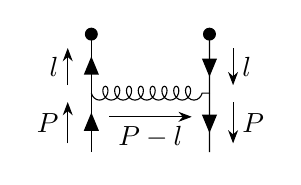
\begin{tikzpicture}[baseline=($(a)!0.5!(exa)$.base)]
		\begin{feynman}
			\node[dot] (a);
			\node[right=\FDWidthS of a,dot] (b);
			\vertex[below=\FDHeightS of a] (exa);
			\vertex[below=\FDHeightS of b] (exb);
			\vertex at ($(exa)!0.5!(a)$) (a1);
			\vertex at ($(exb)!0.5!(b)$) (b1);
			\diagram*{
			% (a) --[Eikonal] (b);
			(exa) --[fermion,momentum=\(P\)] (a1) --[fermion,momentum=\(l\)] (a);
			(b) --[fermion,momentum=\(l\)] (b1) --[fermion,momentum=\(P\)] (exb);
			(a1) --[gluon,momentum'=\(P-l\)] (b1);
			};
		\end{feynman}
	\end{tikzpicture} & =\frac{1}{2}\bar u(P) \pqty{-ig_st^a\gamma_\nu} \int\mm{l}\frac{i}{\slashed l-m+i\epsilon}\gamma^+\frac{-ig^{\mu \nu}}{(P-l)^2+i\epsilon} \frac{i}{\slashed l-m+i\epsilon}\pqty{-ig_s\gamma_{\mu}t^a}u(P)\delta(l^z-xP^z)\notag \\
	                            & =-i\frac{g_s^2C_F}{2}\int\mm{l}\bar u(P) \gamma^\mu \frac{\slashed l+m}{l^2-m^2+i\epsilon}\gamma^+\frac{\slashed l+m}{l^2-m^2+i\epsilon}\gamma_{\mu} u(P)\frac{1}{(P-l)^2+i\epsilon}\delta(l^z-xP^z)
\end{align}
After spin sum:
\begin{align}
	\frac{1}{2}\sum_s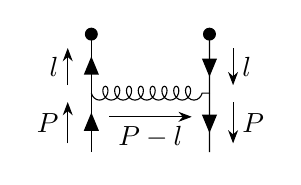
\begin{tikzpicture}[baseline=($(a)!0.5!(exa)$.base)]
		\begin{feynman}
			\node[dot] (a);
			\node[right=\FDWidthS of a,dot] (b);
			\vertex[below=\FDHeightS of a] (exa);
			\vertex[below=\FDHeightS of b] (exb);
			\vertex at ($(exa)!0.5!(a)$) (a1);
			\vertex at ($(exb)!0.5!(b)$) (b1);
			\diagram*{
			% (a) --[Eikonal] (b);
			(exa) --[fermion,momentum=\(P\)] (a1) --[fermion,momentum=\(l\)] (a);
			(b) --[fermion,momentum=\(l\)] (b1) --[fermion,momentum=\(P\)] (exb);
			(a1) --[gluon,momentum'=\(P-l\)] (b1);
			};
		\end{feynman}
	\end{tikzpicture} & =\frac{-ig_s^2C_F}{4}\int\mm{l}\sum_s\bar u(P) \gamma^\mu \frac{\slashed l+m}{l^2-m^2+i\epsilon}\gamma^+\frac{\slashed l+m}{l^2-m^2+i\epsilon}\gamma_{\mu} u(P)\frac{1}{(P-l)^2+i\epsilon}\delta(l^z-xP^z)\notag \\
	                                             & =\frac{-ig_s^2C_F}{4}\int\mm{l} \frac{\Tr{(\slashed P+m)\gamma^\mu(\slashed l+m)\gamma^+(\slashed l+m)\gamma_{\mu}}}{(l^2-m^2+i\epsilon)^2(P-l)^2}\delta(l^z-xP^z)
\end{align}

\section{Matching to PDF}
The matching coefficient $Z$ is defined as
\begin{align}
	\tilde{q}(x)=\int_{0}^{1} \frac{d y}{y} Z\left(\frac{x}{y}, \frac{P^{z}}{\mu}\right) q(y)+\mathcal{O}\left(\frac{\Lambda_{Q C D}^{2}}{P_{z}^{2}}, \frac{M^{2}}{P_{z}^{2}}\right)
\end{align}
For leading order, it's
\begin{align}
	\delta(1-x)=\int_0^1\frac{\dd y}{y}Z\pqty{\frac{x}{y},\frac{P^z}{\mu}}\delta(1-y)
\end{align}
It's straightforward to get (under the assumption that the heaviside theta function $\theta(0)=0$)
\begin{align}
	Z\pqty{\frac{x}{y},\frac{P^z}{\mu}}=\delta\pqty{1-\frac{x}{y}}
\end{align}
The one loop matching factor is
\begin{align}
	  & \left(1+\delta \tilde{Z}_{F}\right) \delta(1-x)+\tilde{q}^{(1)}(x)
	= \int_{0}^{1} \frac{d y}{y}\left[\delta\left(\frac{x}{y}-1\right)+Z^{(1)}\left(\frac{x}{y}, \frac{p^{z}}{\mu}\right)\right]\left[\left(1+\delta Z_{F}\right) \delta(1-y)+q^{(1)}(y)\right]
\end{align}
where $Z_F$ is independent of $x$ and $y$. In axial gauge, $Z_F$ is the fermion self energy, while in Feynman gauge, it's the combination of fermion self energy, gauge link self energy and loops between quark line and gauge link line involving only one side of the uncut diagram. Up to one loop the equation becomes
\begin{align*}
	\left(1+\delta \tilde{Z}_{F}\right) \delta(1-x)+\tilde{q}^{(1)}(x)
	  & = \int_{0}^{1} \frac{d y}{y}\left[\delta\left(\frac{x}{y}-1\right)\left(1+\delta Z_{F}\right) \delta(1-y)+\delta\left(\frac{x}{y}-1\right)q^{(1)}(y)+Z^{(1)}\left(\frac{x}{y}, \frac{p^{z}}{\mu}\right) \delta(1-y)\right] \\
	% \left(1+\delta \tilde{Z}_{F}\right) \delta(1-x)+\tilde{q}^{(1)}(x)
	  & = \left(1+\delta Z_{F}\right) \delta(1-x)+q^{(1)}(x)\theta(x)\theta(1-x)+Z^{(1)}\left(x, \frac{p^{z}}{\mu}\right)
\end{align*}

We then have (note that the momentum fraction $x$ of PDF can't exceed $(0,1)$)
\begin{align}
	\delta \tilde{Z}_{F} \delta(1-x)+\tilde{q}^{(1)}(x) & = \delta Z_{F}\delta(1-x)+q^{(1)}(x)+Z^{(1)}\left(x, \frac{p^{z}}{\mu}\right)                          \\
	Z^{(1)}\left(x, \frac{p^{z}}{\mu}\right)            & =\left[\delta \tilde{Z}_{F}-\delta Z_{F}\right] \delta(1-x)+\left[\tilde{q}^{(1)}(x)-q^{(1)}(x)\right]
\end{align}
$\delta Z_F$ and $\delta \tilde Z_F$ combined with delta functions are to be merged into $q^{(1)}$ and $\tilde q^{(1)}$ and becomes plus distribution.

At two loop, we're looking at
\begin{align}
	  & \left(1+\delta \tilde{Z}_{F}^{(1)}+\delta \tilde{Z}_{F}^{(2)}\right) \delta(1-x)+\tilde{q}^{(1)}(x)+\tilde{q}^{(2)}(x)\notag \\&
	= \int_{0}^{1} \frac{d y}{y}\left[\delta\left(\frac{x}{y}-1\right)+Z^{(1)}\left(\frac{x}{y}, \frac{p^{z}}{\mu}\right)+Z^{(2)}\left(\frac{x}{y}, \frac{p^{z}}{\mu}\right)\right]\left[\left(1+\delta Z_{F}^{(1)}+\delta Z_{F}^{(2)}\right) \delta(1-y)+q^{(1)}(y)+q^{(2)}(y)\right]
\end{align}
Then
\begin{align}
	  & \left(1+\delta \tilde{Z}_{F}^{(1)}+\delta \tilde{Z}_{F}^{(2)}\right) \delta(1-x)+\tilde{q}^{(1)}(x)+\tilde{q}^{(2)}(x)\notag                                                                                                                                                                     \\
	= & \int_{0}^{1} \frac{d y}{y}\Bqty{\delta\left(\frac{x}{y}-1\right)\left[\left(1+\delta Z_{F}^{(1)}+\delta Z_{F}^{(2)}\right) \delta(1-y)+q^{(1)}(y)+q^{(2)}(y)\right]\notag                                                                                                                        \\&\hspace*{1in}+\left[\left(1+\delta Z_{F}^{(1)}\right) \delta(1-y)+q^{(1)}(y)\right]Z^{(1)}\left(\frac{x}{y}, \frac{p^{z}}{\mu}\right)+Z^{(2)}\left(\frac{x}{y}, \frac{p^{z}}{\mu}\right)\delta(1-y)}\delta(1-y)\notag\\
	= & \left(1+\delta Z_{F}^{(1)}+\delta Z_{F}^{(2)}\right) \delta(1-x)+q^{(1)}(x)+q^{(2)}(x)+\left(1+\delta Z_{F}^{(1)}\right)Z^{(1)}\left(x, \frac{p^{z}}{\mu}\right)+\int_{0}^{1} \frac{d y}{y}q^{(1)}(y)Z^{(1)}\left(\frac{x}{y}, \frac{p^{z}}{\mu}\right)+Z^{(2)}\left(x, \frac{p^{z}}{\mu}\right) \\
	= & \left(1+\delta Z_{F}^{(1)}+\delta Z_{F}^{(2)}\right) \delta(1-x)+q^{(1)}(x)+q^{(2)}(x)
	+\left(1+\delta Z_{F}^{(1)}\right)\Bqty{\left[\delta \tilde{Z}_{F}^{(1)}-\delta Z_{F}^{(1)}\right] \delta(1-x)+\left[\tilde{q}^{(1)}(x)-q^{(1)}(x)\right]}\notag\\&\hspace*{1in}
	+\int_{0}^{1} \frac{d y}{y}q^{(1)}(y)\Bqty{\left[\delta \tilde{Z}_{F}^{(1)}-\delta Z_{F}^{(1)}\right] \delta(1-\frac{x}{y})+\left[\tilde{q}^{(1)}\left(\frac{x}{y}\right)-q^{(1)}\left(\frac{x}{y}\right)\right]}
	+Z^{(2)}\left(x, \frac{p^{z}}{\mu}\right)\notag\\
	= & \left(1+\delta Z_{F}^{(1)}+\delta Z_{F}^{(2)}\right) \delta(1-x)+q^{(1)}(x)+q^{(2)}(x)
	+\left(1+\delta Z_{F}^{(1)}\right)\Bqty{\left[\delta \tilde{Z}_{F}^{(1)}-\delta Z_{F}^{(1)}\right] \delta(1-x)+\left[\tilde{q}^{(1)}(x)-q^{(1)}(x)\right]}\notag\\&\hspace*{1in}
	+q^{(1)}(x)\left[\delta \tilde{Z}_{F}^{(1)}-\delta Z_{F}^{(1)}\right]+\int_{0}^{1} \frac{d y}{y}q^{(1)}(y)\left[\tilde{q}^{(1)}\left(\frac{x}{y}\right)-q^{(1)}\left(\frac{x}{y}\right)\right]
	+Z^{(2)}\left(x, \frac{p^{z}}{\mu}\right)\notag\\
	= & \left(1+\delta Z_{F}^{(1)}+\delta Z_{F}^{(2)}\right) \delta(1-x)+\tilde{q}^{(1)}(x)+q^{(2)}(x)
	+\left(1+\delta Z_{F}^{(1)}\right)\left[\delta \tilde{Z}_{F}^{(1)}-\delta Z_{F}^{(1)}\right] \delta(1-x)+\delta Z_{F}^{(1)}\tilde{q}^{(1)}(x)\notag\\&\hspace*{1in}
	-\left(2\delta Z_{F}^{(1)}-\delta \tilde{Z}_{F}^{(1)}\right)q^{(1)}(x)+\int_{0}^{1} \frac{d y}{y}q^{(1)}(y)\left[\tilde{q}^{(1)}\left(\frac{x}{y}\right)-q^{(1)}\left(\frac{x}{y}\right)\right]
	+Z^{(2)}\left(x, \frac{p^{z}}{\mu}\right)
\end{align}
and this concludes to
\begin{align}
	Z^{(2)}\left(x, \frac{p^{z}}{\mu}\right) & =
	\begin{aligned}[t]
		\left(1+\delta \tilde{Z}_{F}^{(1)}+\delta \tilde{Z}_{F}^{(2)}\right) \delta(1-x)+\tilde{q}^{(1)}(x)+\tilde{q}^{(2)}(x)-\left(1+\delta Z_{F}^{(1)}+\delta Z_{F}^{(2)}\right) \delta(1-x)-q^{(1)}(x)-q^{(2)}(x)&\\-\left(1+\delta Z_{F}^{(1)}\right)Z^{(1)}\left(x, \frac{p^{z}}{\mu}\right)-\int_{0}^{1} \frac{d y}{y}q^{(1)}(y)Z^{(1)}\left(\frac{x}{y}, \frac{p^{z}}{\mu}\right)&
	\end{aligned}\NL
	                                         & =\begin{aligned}[t]
		\left(\delta \tilde{Z}_{F}^{(1)}-\delta Z_{F}^{(1)}+\delta \tilde{Z}_{F}^{(2)}-\delta Z_{F}^{(2)}\right) \delta(1-x)+\tilde{q}^{(1)}(x)-q^{(1)}(x)+\tilde{q}^{(2)}(x)-q^{(2)}(x)&\\-\left(1+\delta Z_{F}^{(1)}\right)Z^{(1)}\left(x, \frac{p^{z}}{\mu}\right)-\int_{0}^{1} \frac{d y}{y}q^{(1)}(y)Z^{(1)}\left(\frac{x}{y}, \frac{p^{z}}{\mu}\right)&
	\end{aligned}       \\
	                                         & =\begin{aligned}[t]
		                                                                                                                                                                                                                                                                                                        & \left(\delta \tilde{Z}_{F}^{(1)}+\delta \tilde{Z}_{F}^{(2)}-\delta Z_{F}^{(1)}-\delta Z_{F}^{(2)}\right) \delta(1-x)+\tilde{q}^{(1)}(x)-q^{(1)}(x)+\tilde{q}^{(2)}(x)-q^{(2)}(x)+\delta Z_{F}^{(1)}\tilde{q}^{(1)}(x) \\&
		-\left(2\delta Z_{F}^{(1)}-\delta \tilde{Z}_{F}^{(1)}\right)q^{(1)}(x)+\left(1+\delta Z_{F}^{(1)}\right)\left[\delta \tilde{Z}_{F}^{(1)}-\delta Z_{F}^{(1)}\right] \delta(1-x)+\int_{0}^{1} \frac{d y}{y}q^{(1)}(y)\left[\tilde{q}^{(1)}\left(\frac{x}{y}\right)-q^{(1)}\left(\frac{x}{y}\right)\right] &
	\end{aligned}\notag \\
	                                         & =\begin{aligned}[t]
		                                                                                                                                                                                                                                                                                                        & \left(\delta \tilde{Z}_{F}^{(1)}-\delta Z_{F}^{(1)}+\delta \tilde{Z}_{F}^{(2)}-\delta Z_{F}^{(2)}\right) \delta(1-x)+\tilde{q}^{(1)}(x)-q^{(1)}(x)+\tilde{q}^{(2)}(x)-q^{(2)}(x)+\delta Z_{F}^{(1)}\tilde{q}^{(1)}(x) \\&
		-\left(2\delta Z_{F}^{(1)}-\delta \tilde{Z}_{F}^{(1)}\right)q^{(1)}(x)+\left(1+\delta Z_{F}^{(1)}\right)\left[\delta \tilde{Z}_{F}^{(1)}-\delta Z_{F}^{(1)}\right] \delta(1-x)+\int_{0}^{1} \frac{d y}{y}q^{(1)}(y)\left[\tilde{q}^{(1)}\left(\frac{x}{y}\right)-q^{(1)}\left(\frac{x}{y}\right)\right] &
	\end{aligned}\notag \\
\end{align}

\appendix
\section{Conventions\label{sec:conv}}
The quark field $\psi$ reads
\begin{align}
	\psi(x)=\int \frac{\dd^{3} \vec{k}}{(2 \pi)^{3}} \frac{1}{2 E_{k}}\left[u(k) e^{-i k \cdot x} b_{k}+v(k)e^{ik\cdot x} d_{k}^{\dagger}\right]
\end{align}
and the projection of single particle state is
\begin{align}
	\ket{p}=b_p^{\dagger}\ket{0}
\end{align}
\begin{align}
	\Bqty{b_{\vb{p}}^r,b_{\vb{q}}^{s\dagger}}=(2\pi)^32E\delta^{(3)}(\vb{p}-\vb{q})\delta^{rs}
\end{align}
The Dirac spinor is normalized to
\begin{align}
	\bar u^s(p) u(p)=2m\delta^{rs}
\end{align}
With Gordon identity, one can derive\cite{Srednicki2007}
\begin{align}
	\bar u(P) \gamma^\mu u(P) =2P^\mu
\end{align}
The axial gauge propagator is
\begin{align}
	\tilde D_G^{A\mu\nu}(p)=-i \delta_{a b}\left(g^{\mu \nu}-\frac{n^{\mu} p^{\nu}+n^{\nu} p^{\mu}}{n \cdot p}+n \cdot n \frac{p^{\mu} p^{\nu}}{(n \cdot p)^{2}}\right) \frac{1}{p^{2}}
\end{align}
The Feynman gauge propagator is
\begin{align}
	\tilde D_G^{F\mu\nu}(p)= \frac{-i g^{\mu\nu} \delta_{a b}}{p^{2}+i\epsilon}
\end{align}
State contract with field:
\begin{align}
	\wick{\c{\psi}(x)\c{\ket{P}}} & =\int\mme{l}\frac{1}{2E_{\vb{l}}}\bqty{b_{\vb{l}}u(l)e^{-il\cdot x}+d_{\vb{l}}^{\dagger}v(l)e^{il\cdot x}}b_{\vb{P}}^{\dagger}\ket{0}\notag \\
	                              & =\int\mme{l}\frac{1}{2E_{\vb{l}}}u(l)e^{-il\cdot x}(2\pi)^32E\delta^{(3)}(\vb{l}-\vb{P})\ket{0}\notag                                       \\
	                              & =u(P)e^{-iP\cdot x}
\end{align}
and correspondingly
\begin{align}
	\wick{\c{\bra{P}}\c{\bar\psi}(x)} & =\bar u(P)e^{iP\cdot x}
\end{align}
Plus function is defined as\cite{Collins2009}
\begin{align}
	\int_{0}^{1} \mathrm{d} x\left(\frac{1}{1-x}\right)_{+} T(x) \equiv \int_{0}^{1} \mathrm{d} x \frac{T(x)-T(1)}{1-x}
\end{align}
\begin{align}
	\int_{0}^{1} \mathrm{d} x \frac{A(x)}{(1-x)_{+}} T(x) \equiv \int_{0}^{1} \mathrm{d} x \frac{A(x) T(x)-A(1) T(1)}{1-x}
\end{align}
The plus function could also be defined in a different fashion:
\begin{align}
	F_{+}(x):=\lim _{\beta \rightarrow 0}\left(F(x) \theta(1-\beta-x)-\delta(1-\beta-x) \int_{0}^{1-\beta} \dd y F(y)\right)
\end{align}
and with a smooth test function it's defined the same way as above:
\begin{align}
	\int_{0}^{1} \dd x F_{+}(x) G(x)=\int_{0}^{1} \dd x F(x)[G(x)-G(1)]
\end{align}
with
\begin{align}
	\int_{0}^{1} \dd x F(x)_{+}=0
\end{align}
For a flexible lower boundary:
\begin{align}
	\int_{a}^{1} \dd x F_{+}(x) G(x)=\int_{a}^{1} \dd x F(x)[G(x)-G(1)]+G(1) \int_{0}^{a} \dd x F(x)
\end{align}
Also if rule out some smoothness problem
\begin{align}
	[f(x)]_{+}=f(x)-\delta(1-x) \int_{0}^{1} f(z) \mathrm{d} z
\end{align}
Here we use a modified version of plus function (to not confuse this with those used in \cite{Stewart:2017tvs}, we use boxplus for a plus function with integration limit from minus infinity to plus infinity)
\begin{align}
	f_{\boxplus}(x) & =f(x)-\delta(1-x)\int_{-\infty}^\infty\dd yf(y)       \\
	                & =f(x)-\delta(1-x)\int_{-\infty}^\infty\dd l^zf(y)/P^z
\end{align}
For functions as
\begin{align}
	\pqty{\frac{1}{1-x}}^{1-\epsilon}
\end{align}
instead of expanding them in $\epsilon->0$ limit, we can treat them as distributions and expand them into the combinations of delta functions and plus functions.
\begin{align}
	\pqty{\frac{1}{1-x}}^{1-\epsilon}&=\pqty{\frac{1}{1-x}}^{1-\epsilon}_++\delta(1-x)\int_0^1\pqty{\frac{1}{1-z}}^{1-\epsilon}\dd z\\
	&=\pqty{\frac{1}{1-x}}^{1-\epsilon}_++\frac{\delta(1-x)}{\epsilon}\\
	&=\pqty{\frac{1}{1-x}}_++\frac{\delta(1-x)}{\epsilon}
\end{align}
and
\begin{align}
	\pqty{\frac{1}{1-x}}^{1-\epsilon}&=\pqty{\frac{1}{1-x}}^{1-\epsilon}_{\boxplus}+\delta(1-x)\int_{-\infty}^{\infty}\pqty{\frac{1}{1-z}}^{1-\epsilon}\dd z\\
	&=\pqty{\frac{1}{1-x}}^{1-\epsilon}_{\boxplus}+0\frac{\delta(1-x)}{\epsilon}\\
\end{align}

The convention for path ordering is that the field with higher value of the integration variable $s$ goes to the left.

The definition of Heaviside theta function follows
\begin{align}
	\theta(z)=\int\frac{\dd w}{2\pi}\frac{ie^{-iwz }}{w+i\epsilon}
\end{align}
and here we choose
\begin{align}
	\theta(0)=1
\end{align}

\section{Wick Contraction: Axial Gauge\label{sec:WickA}}
Take diagram \ref{1b} as an example
\begin{center}
	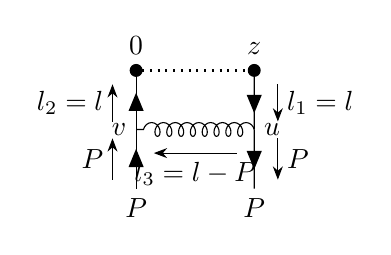
\begin{tikzpicture}[baseline=($(a)!0.5!(exa)$.base)]
		\begin{feynman}
			\node[dot, label=above:\(0\)] (a);
			\node[right=\FDWidth of a,dot, label=above:\(z\)] (b);
			\vertex[below=\FDHeight of a, label=below:\(P\)] (exa);
			\vertex[below=\FDHeight of b, label=below:\(P\)] (exb);
			\vertex[label=left:\(v\)] at ($(exa)!0.5!(a)$) (a1);
			\vertex[label=right:\(u\)] at ($(exb)!0.5!(b)$) (b1);
			\diagram*{
			(a) --[ghost] (b);
			(exa) --[fermion,momentum=\(P\)] (a1) --[fermion,momentum={\(l_2=l\)}] (a);
			(b) --[fermion,momentum={\(l_1=l\)}] (b1) --[fermion,momentum=\(P\)] (exb);
			(b1) --[gluon,momentum={\(l_3=l-P\)}] (a1);
			};
		\end{feynman}
	\end{tikzpicture}
\end{center}
This corresponds to
\begin{align}
	  & \frac{1}{4 \pi} \int \dd z e^{i x P^{z} z}\wick[offset=1.3em]{\langle \c1 P|\int\dd^4u\c1{\bar\psi}_u}\wick{\c1{\psi}_u \c2{A}_u\c1{\bar{\psi}}(z) \gamma^{z}\c3{\psi}(0)\int\dd^4v\c3{\bar\psi}_v\c4{\psi}_v \c2{A}_v| \c4 P\rangle} \\
	= & \frac{1}{4 \pi} \int \dd z e^{i x P^{z} z}\int\dd^4u\dd^4v\bar u(P)e^{iP\cdot u}\int\mm{l_1}\tilde D_F(l_1)e^{-il_1\cdot (u-z)}\gamma^z\int\mm{l_2}\tilde D_F(l_2)e^{-il_2\cdot (-v)}\notag                                           \\&\int\mm{l_3}\tilde D_G(l_3)e^{-il_3\cdot (v-u)}u(P)e^{-iP\cdot v}\\
	= & \frac{1}{4 \pi} \int \dd z\int\dd^4u\dd^4v \int\mm{l_1}\int\mm{l_2}\int\mm{l_3}e^{i x P^{z} z+il_1\cdot z}e^{i(P-l_1+l_3)\cdot u}e^{i(l_2-l_3-P)\cdot v}\bar u(P)\tilde D_F(l_1)\gamma^z\tilde D_F(l_2)\notag                         \\&\tilde D_G(l_3)u(P)\\
	= & \frac{1}{4 \pi} \int \dd z \int\mm{l}e^{i x P^{z} z+il\cdot z}\bar u(P)\tilde D_F(l)\gamma^z\tilde D_F(l)\tilde D_G(l-P)u(P)                                                                                                          \\
	= & \frac{1}{4 \pi} \int \dd z \int\mm{l}e^{i (x P^{z} -l^z) z}\bar u(P)\tilde D_F(l)\gamma^z\tilde D_F(l)\tilde D_G(l-P)u(P)                                                                                                             \\
	= & \frac{1}{4 \pi} \int\mmd[1]{l^0}\int\mmd[2]{\vb{l}_T}\eval{\bar u(P)\tilde D_F(l)\gamma^z\tilde D_F(l)\tilde D_G(l-P)u(P)}_{l^z=xP^z}
\end{align}
where
\begin{align}
	\int \dd z e^{i (x P^{z} -l^z) z}=2\pi\delta(l^z-xP^z)
\end{align}
This indicates what the Feynman diagram actually means: a normal Feynman diagram with only 3-momentum integration, where the axial momentum is fixed by $l^z=xP^z$, and with an extra $1/4\pi$ factor.

\section{Wick Contraction: Feynman Gauge\label{sec:WickF}}
\subsection{Normal Diagrams}
Let's take diagram~\ref{2`-} as an example:
\begin{center}
	\begin{tikzpicture}[baseline=($(a)!0.5!(exa)$.base)]
		\begin{feynman}
			\node[dot] (a);
			\node[right=\FDWidth of a,dot] (b);
			\vertex at ($(a)!0.5!(b)$) (o);
			\vertex[below=\FDHeight of a] (exa);
			\vertex[below=\FDHeight of b] (exb);
			\vertex at ($(exa)!0.5!(a)$) (a1);
			\vertex at ($(exb)!0.5!(b)$) (b1);
			\diagram*{
			(o) --[Eikonal,rmomentum=\(P-l\)] (b);
			(exa) --[fermion,momentum=\(P\)] (a);
			(b) --[fermion,momentum=\(l\)] (b1) --[fermion,momentum=\(P\)] (exb);
			(o) --[gluon,momentum'=\(P-l\)] (b1);
			};
		\end{feynman}
	\end{tikzpicture}
\end{center}
The one loop quasi PDF is
\begin{align}
	\tilde{q}^{(1)}_1(x)=\frac{1}{2} \int \frac{\dd z}{2 \pi} e^{i x P^{z} z}\langle P, S|\int\dd^4u\pqty{-ig_st^a\gamma_{\mu}}\bar\psi_u\psi_u A_u^{\mu}\bar{\psi}(z) \gamma^z \tilde{\mathcal{W}}[z, 0]  \psi(0)| P, S\rangle
\end{align}
where
\begin{align}
	\tilde{\mathcal{W}}[z, 0] =\mathcal{P} \exp\left[-i g_s \int_{0}^{z} \dd z^{\prime} A^{a,z}\left(z^{\prime}\right) \mathrm{t}^{a}\right]
\end{align}
We should rewrite the gauge link to the product of two gauge links connect to infinity
\begin{align}
	\tilde{\mathcal{W}}[z, 0] =\tilde{\mathcal{W}}[z, +\infty] \tilde{\mathcal{W}}[\infty, 0]
\end{align}
and in one loop level it equals to
\begin{align*}
	\mathcal{P} \exp\left[i g_s\int_{\infty}^{z} \dd z^{\prime} A^{a,z}\left(z^{\prime}\right) \mathrm{t}^{a}\right]\mathcal{P} \exp\left[i g_s\int_{0}^{\infty} \dd z^{\prime} A^{a,z}\left(z^{\prime}\right) \mathrm{t}^{a}\right]
	=\left[i g_s \mathcal{P} \int_{0}^{\infty} \dd z^{\prime} A^{a,z}\left(z^{\prime}+z\right) \mathrm{t}^{a}\right]-\left[i g_s \mathcal{P} \int_0^{\infty} \dd z^{\prime} A^{a,z}\left(z^{\prime}\right) \mathrm{t}^{a}\right]
\end{align*}
The path ordering gives
\begin{align}
	\mathcal{P} \int_{0}^{\infty} \dd z^{\prime} A^{a,z}\left(z^{\prime}\right) = \int \dd z^{\prime} A^{a,z}\left(z^{\prime}\right)\theta(z')=\int \dd z^{\prime} A^{a,z}\left(z^{\prime}\right)\int\frac{\dd w}{2\pi}\frac{ie^{-iwz' }}{w+i\epsilon}
\end{align}
and
\begin{align}
	\mathcal{P} \bqty{\int_{0}^{\infty} \dd z^{\prime} A^{a,z}\left(z^{\prime}\right)}^2 = \int \dd z^{\prime} A^{a,z}\left(z^{\prime}\right)\theta(z')\int \dd z^{\prime\prime} A^{a,z}\left(z^{\prime\prime}\right)\theta(z''-z')
\end{align}
with all momenta involved with $z'$ must be in the $z$-direction (the exponent is actually $z'n\cdot w$ if a four-vector $w$ actually exists). Consider the second gauge link first, the matrix element is then (discarding all couplings)
\begin{align*}
	  & \langle P, S|\bar\psi_u\psi_u A_u^{\mu}\bar{\psi}(z) \gamma^z \int \dd z^{\prime} A^{a,z}\left(z^{\prime}+z\right) \int\frac{\dd w}{2\pi}\frac{ie^{-iwz' }}{w+i\epsilon}\psi(0)| P, S\rangle                                                    \\
	= & \int\dd^4u\langle P, S|\bar\psi_u\psi_u A_u\bar{\psi}(z) \gamma^z \int \dd z^{\prime} A^{a,z}\left(z^{\prime}+z\right) \psi(0)| P, S\rangle\int\frac{\dd w}{2\pi}\frac{ie^{-iwz' }}{w+i\epsilon}                                                \\
	= & \int\dd^4u\wick{\c1{\langle P, S|}\c1{\bar\psi}_u\c2{\psi}_u \c3{A}_u\c2{\bar{\psi}}(z) \gamma^z \int \dd z^{\prime} \c3{A}^{a,z}\left(z^{\prime}+z\right) \c4{\psi}(0)\c4{| P, S\rangle}}\int\frac{\dd w}{2\pi}\frac{ie^{-iwz' }}{w+i\epsilon} \\
	= & \int \dd z^{\prime}\int\dd^4u \bar u(P)e^{iP\cdot u}\int\mm{l_1}\tilde D_F(l_1)e^{-il_1\cdot(u-z)}\gamma^z \int\mm{l_2}\tilde D_G(l_2)e^{-il_2\cdot(u-z'-z)}u(P)\int\frac{\dd w}{2\pi}\frac{ie^{-iwz' }}{w+i\epsilon}                           \\
	= & \int \dd z^{\prime}\int\dd^4u \int\mm{l_1}\int\mm{l_2}\int\frac{\dd w}{2\pi}\bar u(P)e^{i(P-l_1-l_2)\cdot u}e^{i(l_1+l_2)\cdot z}e^{-iwz' -il_2\cdot z'}\tilde D_F(l_1)\gamma^z \tilde D_G(l_2)u(P)\frac{i}{w+i\epsilon}                        \\
	= & \int \dd z^{\prime}\int\mm{l}\int\frac{\dd w}{2\pi}\bar u(P)e^{iP\cdot z}e^{-iwz' +i(P-l)^z z'}\tilde D_F(l)\gamma^z \tilde D_G(P-l)u(P)\frac{i}{w+i\epsilon}                                                                                   \\
	= & \bar u(P)e^{iP\cdot z}\int\mm{l}\tilde D_F(l)\gamma^z \tilde D_G^{\mu z}(P-l)\frac{i}{P^z-l^z+i\epsilon}u(P)
\end{align*}
The complete quasi PDF at one loop is
\begin{align}
	  & \frac{g_s^2C_F}{2} \int \frac{\dd z}{2 \pi} e^{i x P^{z} z}\bar u(P)\gamma_{\mu}e^{iP\cdot z}\int\mm{l}\tilde D_F(l)\gamma^z \tilde D_G^{\mu z}(P-l)\frac{i}{P^z-l^z+i\epsilon}u(P)\notag \\
	= & \frac{g_s^2C_F}{2 P^z}\bar u(P)\gamma_{\mu}\int\mm{l}\tilde D_F(l)\gamma^z \tilde D_G^{\mu z}(P-l)\frac{i}{P^z-l^z+i\epsilon}u(P)\delta(1-x)\notag
\end{align}
multiplied by those couplings. This basically established that the momentum of a gluon equals to the momentum of the eikonal line it attaches to. We then have the Feynman rule:
\begin{align}
	\feynmandiagram[small, horizontal=a to b,baseline=(a.base)]{
	a[dot] --[Eikonal,momentum=\(k\)] b;
	};=\frac{i}{n\cdot k+i\epsilon};\qquad
	\feynmandiagram[small, horizontal=a to b,baseline=(a.base)]{
	a --[Eikonal,rmomentum=\(k\)] b[dot];
	};=\frac{i}{n\cdot k+i\epsilon}
\end{align}
and for the gluon-eikonal vertex on the r.h.s., an extra minus sign is added for the normal $(-ig_st^a)$.

\subsection{Gauge Link Self Energy Related Diagrams}
The next job is to determine the Feynman rule for
\begin{center}
	\begin{tikzpicture}[baseline=($(a)!0.5!(exa)$.base)]
		\begin{feynman}
			\node[dot] (a);
			\node[right=\FDWidth of a,dot] (b);
			\vertex at ($(a)!0.3!(b)$) (o1);
			\vertex at ($(a)!0.7!(b)$) (o2);
			\vertex[below=\FDHeight of a] (exa);
			\vertex[below=\FDHeight of b] (exb);
			\diagram*{
			(a) --[Eikonal,momentum=\(l\)] (o1);
			(b) --[Eikonal,momentum'=\(-l\)] (o2);
			(exa) --[fermion,momentum=\(P\)] (a);
			(b) --[fermion,momentum=\(P\)] (exb);
			(o1) --[gluon, half right,momentum'=\(l\)] (o2);
			};
		\end{feynman}
	\end{tikzpicture}\text{\qquad \&\qquad }
	\begin{tikzpicture}[baseline=($(a)!0.5!(exa)$.base)]
		\begin{feynman}
			\node[dot] (a);
			\node[right=\FDWidth of a,dot] (b);
			\vertex at ($(a)!0.6!(b)$) (o);
			\vertex at ($(a)!0.3!(b)$) (o1);
			\vertex at ($(a)!0.8!(b)$) (o2);
			\vertex[below=\FDHeight of a] (exa);
			\vertex[below=\FDHeight of b] (exb);
			\diagram*{
			(a) --[Eikonal,momentum=\(l\)] (o1) --[Eikonal,rmomentum=\(l\)] (o);
			(exa) --[fermion,momentum=\(P\)] (a);
			(b) --[fermion,momentum=\(P\)] (exb);
			(o1) --[gluon, half right,momentum'=\(l\)] (o);
			};
		\end{feynman}
	\end{tikzpicture}
\end{center}
The first one is
\begin{align}
	\frac{1}{2} \int \frac{\dd z}{2 \pi} e^{i x P^{z} z}\langle P, S|\bar{\psi}(z) \gamma^z \left[i g_s \mathcal{P} \int_0^{\infty} \dd z^{\prime} A^{a,z}\left(z^{\prime}+z\right) \mathrm{t}^{a}\right]\left[-i g_s \mathcal{P} \int_{0}^{\infty} \dd z^{\prime} A^{a,z}\left(z^{\prime}\right) \mathrm{t}^{a}\right]  \psi(0)| P, S\rangle
\end{align}
Let's look at the coupling-free form:
\begin{align*}
	  & \int \frac{\dd z}{2 \pi} e^{i x P^{z} z}\langle P, S|\bar{\psi}(z) \gamma^z \left[ \mathcal{P} \int_0^{\infty} \dd z^{\prime} A^{a,z}\left(z^{\prime}+z\right) \right]\left[ \mathcal{P} \int_{0}^{\infty} \dd z^{\prime\prime} A^{a,z}\left(z^{\prime\prime}\right) \right]  \psi(0)| P, S\rangle \\
	= & \int \frac{\dd z}{2 \pi} e^{i x P^{z} z}\langle P, S|\bar{\psi}(z) \gamma^z
	\int \dd z^{\prime} A^{a,z}\left(z^{\prime}+z\right)
	\int \dd z^{\prime\prime} A^{a,z}\left(z^{\prime\prime}\right)  \psi(0)| P, S\rangle\int\frac{\dd w}{2\pi}\frac{ie^{-iwz' }}{w+i\epsilon}\int\frac{\dd h}{2\pi}\frac{ie^{-ihz'' }}{h+i\epsilon}\\
	= & \int \frac{\dd z}{2 \pi} e^{i x P^{z} z}\wick{\langle \c1P, S|\c1{\bar{\psi}}(z) \gamma^z
		\int \dd z^{\prime} \c2A^{a,z}\left(z^{\prime}+z\right)
		\int \dd z^{\prime\prime} \c2A^{a,z}\left(z^{\prime\prime}\right)  \c1\psi(0)| \c1P, S\rangle}\int\frac{\dd w}{2\pi}\frac{ie^{-iwz' }}{w+i\epsilon}\int\frac{\dd h}{2\pi}\frac{ie^{-ihz'' }}{h+i\epsilon}\\
	= & \int \frac{\dd z}{2 \pi} e^{i x P^{z} z}\bar u(P)e^{iP\cdot z}\gamma^z\int\dd z'\dd z''\int\mm{l}\tilde D_G^{zz}(l)e^{-il\cdot(z''-z'-z)}u(P)\int\frac{\dd w}{2\pi}\frac{ie^{-iwz' }}{w+i\epsilon}\int\frac{\dd h}{2\pi}\frac{ie^{-ihz'' }}{h+i\epsilon}                                           \\
	= & \bar u(P)\int \frac{\dd z}{2 \pi} e^{i (x-1) P^{z} z+il^zz}\gamma^z\int\dd z'\dd z''\int\mm{l}\tilde D_G^{zz}(l)\int\frac{\dd w}{2\pi}\frac{i}{w+i\epsilon}\int\frac{\dd h}{2\pi}\frac{i}{h+i\epsilon}e^{-i(w-l)\cdot z'}e^{-i(l+h)\cdot z''} u(P)                                                 \\
	= & \bar u(P)\int \frac{\dd z}{2 \pi} e^{-i (1-x) P^{z} z+il^zz}\gamma^z\int\mm{l}\tilde D_G^{zz}(l)\frac{i}{l^z+i\epsilon}\frac{i}{-l^z+i\epsilon} u(P)                                                                                                                                               \\
	= & \bar u(P)\gamma^z\int\mm{l}\tilde D_G^{zz}(l)\frac{i}{l^z+i\epsilon}\frac{i}{-l^z+i\epsilon}\delta(l^z-(1-x)P^z) u(P)
\end{align*}
One can start with a different route:
\begin{align}
	\bar u(P)\int \frac{\dd z}{2 \pi} e^{-i (1-x) P^{z} z+il^zz}\gamma^z\int\dd z'\dd z''\int\mm{l}\tilde D_G^{zz}(l)\int\frac{\dd w}{2\pi}\frac{i}{w+i\epsilon}\int\frac{\dd h}{2\pi}\frac{i}{h+i\epsilon}e^{-i(w-l)\cdot z'}e^{-i(l+h)\cdot z''} u(P)
\end{align}
The second one is
\begin{align}
	\frac{1}{2} \int \frac{\dd z}{2 \pi} e^{i x P^{z} z}\langle P, S|\bar{\psi}(z) \gamma^z \frac{\mathcal{P} \left[-i g_s \int_{0}^{\infty} \dd z^{\prime} A^{a,z}\left(z^{\prime}\right) \mathrm{t}^{a}\right]\left[-i g_s \int_{0}^{\infty} \dd z^{\prime\prime} A^{a,z}\left(z^{\prime\prime}\right) \mathrm{t}^{a}\right]}{2}  \psi(0)| P, S\rangle
\end{align}
The coupling-free form is\endnote{To check if the sum of theta function can actually leads to unity
	\begin{align*}
		                          & \int\dd zf(z)\bqty{\theta(z-a)+\theta(a-z)}                 \\
		=                         & \int\dd zf(z)\bqty{\glprog{w_1}{(z-a)}+\glprog{w_1}{(a-z)}} \\
		=                         & \int \dd zf(z) e^{\frac{\epsilon  (z-a)}{\text{sgn}(a-z)}}  \\
		\xlongequal{\epsilon\to0} & \int \dd zf(z)
	\end{align*}
}
\begin{align*}
	  & \int \frac{\dd z}{2 \pi} e^{i x P^{z} z}\langle P, S|\bar{\psi}(z) \gamma^z  \mathcal{P} \left[ \int_{0}^{\infty} \dd z^{\prime} A^{a,z}\left(z^{\prime}\right) \int_{0}^{\infty} \dd z^{\prime\prime} A^{a,z}\left(z^{\prime\prime}\right) \right]  \psi(0)| P, S\rangle                                                     \\
	= & \int \frac{\dd z}{2 \pi} e^{i x P^{z} z}\langle P, S|\bar{\psi}(z) \gamma^z \int_{0}^{\infty} \dd z^{\prime} A^{a,z}\left(z^{\prime}\right) \int_{0}^{\infty} \dd z^{\prime\prime} A^{a,z}\left(z^{\prime\prime}\right) \bqty{\theta(z'-z'')+\theta(z''-z')}  \psi(0)| P, S\rangle                                            \\
	= & \int \frac{\dd z}{2 \pi} e^{i x P^{z} z}\langle P, S|\bar{\psi}(z) \gamma^z \int_{0}^{\infty} \dd z^{\prime} A^{a,z}\left(z^{\prime}\right) \int_{0}^{\infty} \dd z^{\prime\prime} A^{a,z}\left(z^{\prime\prime}\right) \psi(0)| P, S\rangle                                                                                  \\
	= & \int \frac{\dd z}{2 \pi} e^{i x P^{z} z}\langle P, S|\bar{\psi}(z) \gamma^z \int \dd z^{\prime} A^{a,z}\left(z^{\prime}\right)\int \dd z^{\prime\prime} A^{a,z}\left(z^{\prime\prime}\right)  \psi(0)| P, S\rangle\int\frac{\dd w}{2\pi}\frac{ie^{-iwz' }}{w+i\epsilon}\int\frac{\dd h}{2\pi}\frac{ie^{-ihz'' }}{h+i\epsilon} \\
	= & \int \frac{\dd z}{2 \pi} e^{i x P^{z} z}\wick{\langle \c1P, S|\c1{\bar{\psi}}(z) \gamma^z \int \dd z^{\prime} \c2A^{a,z}\left(z^{\prime}\right)\int \dd z^{\prime\prime} \c2A^{a,z}\left(z^{\prime\prime}\right)  \c1\psi(0)| \c1P, S\rangle}
	\int\frac{\dd w}{2\pi}\frac{ie^{-iwz' }}{w+i\epsilon}\int\frac{\dd h}{2\pi}\frac{ie^{-ihz'' }}{h+i\epsilon}\\
	= & \int \frac{\dd z}{2 \pi} e^{i x P^{z} z}\bar u(P)e^{iP\cdot z} \gamma^z \int \dd z^{\prime} \int \dd z^{\prime\prime} \int\mm{l}\tilde D_G^{zz}(l)e^{-il\cdot(z''-z')}  u(P)
	\int\frac{\dd w}{2\pi}\frac{ie^{-iwz' }}{w+i\epsilon}\int\frac{\dd h}{2\pi}\frac{ie^{-ihz'' }}{h+i\epsilon}\\
	= & \bar u(P)\int \frac{\dd z}{2 \pi} e^{-i (1-x) P^{z} z} \gamma^z  \int\mm{l}\tilde D_G^{zz}(l)
	\int \dd z^{\prime} \int \dd z^{\prime\prime}\int\frac{\dd w}{2\pi}\frac{i}{w+i\epsilon}\int\frac{\dd h}{2\pi}\frac{i}{h+i\epsilon}e^{-i(w-l)\cdot z'}e^{-i(h+l)\cdot z''} u(P)\\
	= & \bar u(P) \gamma^zu(P) \int \frac{\dd z}{2 \pi} e^{-i (1-x) P^{z} z} \int\mm{l}\tilde D_G^{zz}(l)
	\frac{i}{l^z+i\epsilon}\frac{i}{-l^z+i\epsilon} \\
	= & 2\delta(1-x)\int\mm{l}\tilde D_G^{zz}(l)
	\frac{i}{l^z+i\epsilon}\frac{i}{-l^z+i\epsilon}
\end{align*}
This gives
\begin{align}
	\begin{tikzpicture}[baseline=($(a)!0.5!(exa)$.base)]
		\begin{feynman}
			\node[dot] (a);
			\node[right=\FDWidthS of a,dot] (b);
			\vertex at ($(a)!0.6!(b)$) (o);
			\vertex at ($(a)!0.3!(b)$) (o1);
			\vertex at ($(a)!0.8!(b)$) (o2);
			\vertex[below=\FDHeightS of a] (exa);
			\vertex[below=\FDHeightS of b] (exb);
			\diagram*{
			(a) --[Eikonal,momentum=\(l\)] (o1) --[Eikonal,rmomentum=\(l\)] (o);
			(exa) --[fermion,momentum=\(P\)] (a);
			(b) --[fermion,momentum=\(P\)] (exb);
			(o1) --[gluon, half right,momentum'=\(l\)] (o);
			};
		\end{feynman}
	\end{tikzpicture}=-\frac{g_s^2C_F}{2}\delta(1-x)\int\mm{l}\tilde D_G^{zz}(l)
	\frac{i}{l^z+i\epsilon}\frac{i}{-l^z+i\epsilon}
\end{align}
Let's start from the second line of above derivation and add a small momentum $p$
\begin{align*}
	  & \int_{0}^{\infty} \dd z{'} A^{a,z}\left(z{'}\right) \int_{0}^{\infty} \dd z{''} A^{a,z}\left(z{''}\right) \bqty{\theta(z'-z'')+\theta(z''-z')}                                                                                                                                                                                  \\
	= & \int_{0}^{\infty} \dd z{'} \int_{0}^{\infty} \dd z{''} \int\mm{l}\tilde D_G(l)e^{il^z(z''-z')} \bqty{\int\frac{\dd w}{2\pi}\frac{ie^{-iw(z'-z'') }}{w+i\epsilon}+\int\frac{\dd w}{2\pi}\frac{ie^{-iw(z''-z') }}{w+i\epsilon}}                                                                                                   \\
	= & \int_{0}^{\infty} \dd z{'} \int_{0}^{\infty} \dd z{''} \int\mm{l}\tilde D_G(l) \bqty{\int\frac{\dd w}{2\pi}\frac{ie^{-iw(z'-z'') }e^{il^z(z''-z')}}{w+i\epsilon}+\int\frac{\dd w}{2\pi}\frac{ie^{-iw(z''-z') }e^{-il^z(z''-z')}}{w+i\epsilon}}                                                                                  \\
	= & \int \dd z{'} \int \dd z{''} \int\mm{l}\tilde D_G(l) \bqty{\int\frac{\dd w}{2\pi}\frac{ie^{-iw(z'-z'') }e^{il^z(z''-z')}}{w+i\epsilon}\int\frac{\dd h}{2\pi}\frac{ie^{-ihz'' }}{h+i\epsilon}+\int\frac{\dd w}{2\pi}\frac{ie^{-iw(z''-z') }e^{-il^z(z''-z')}}{w+i\epsilon}\int\frac{\dd h}{2\pi}\frac{ie^{-ihz' }}{h+i\epsilon}} \\
	= & \int \dd z{'} \int \dd z{''} \int\mm{l}\tilde D_G(l) \int\frac{\dd w}{2\pi}\frac{i}{w+i\epsilon}\int\frac{\dd h}{2\pi}\frac{i}{h+i\epsilon}\bqty{e^{-iz'(w+l^z)-iz''(h-w-l^z)}+e^{-iz'(w-l^z)-iz''(h-w+l^z)}}\lim_{p\to0}e^{ipz'}                                                                                               \\
	= & \int \dd z{'} \int \dd z{''} \int\mm{l}\tilde D_G(l) \int\frac{\dd w}{2\pi}\frac{i}{w+i\epsilon}\int\frac{\dd h}{2\pi}\frac{i}{h+i\epsilon}\lim_{p\to0}\bqty{e^{-iz'(w+l^z-p)-iz''(h-w-l^z)}+e^{-iz'(w-l^z-p)-iz''(h-w+l^z)}}                                                                                                   \\
	= & \int\mm{l}\tilde D_G(l) \lim_{p\to0}\bqty{\frac{i}{p-l^z+i\epsilon}\frac{i}{p+i\epsilon}+\frac{i}{p+l^z+i\epsilon}\frac{i}{p+i\epsilon}}                                                                                                                                                                                        \\
	= & \int\mm{l}\tilde D_G(l) \frac{i}{l^z+i\epsilon}\frac{i}{-l^z+i\epsilon}\times 2
\end{align*}
We can reverse the loop momentum of one of the path and add a small inflowing momentum $p$ (in the following diagrams each diagram only represents one specific path, that means the sum of both diagram is the value of the original diagram):
\begin{align*}
	  & \begin{tikzpicture}[baseline=($(a)$.base)]
		\begin{feynman}
			\node[dot] (a);
			\node[right=\FDWidthS of a,dot] (b);
			\vertex at ($(a)!0.6!(b)$) (o);
			\vertex at ($(a)!0.3!(b)$) (o1);
			\vertex at ($(a)!0.8!(b)$) (o2);
			\vertex[below=\FDHeightS of a] (exa);
			\vertex[below=\FDHeightS of b] (exb);
			\diagram*{
			(a) --[Eikonal,momentum=\(p\)] (o1) --[Eikonal,rmomentum=\(l-p\)] (o);
			% (exa) --[fermion,momentum=\(P\)] (a);
			% (b) --[fermion,momentum=\(P\)] (exb);
			(o1) --[gluon, half right,momentum'=\(l\)] (o);
			};
		\end{feynman}
	\end{tikzpicture}+
	\begin{tikzpicture}[baseline=($(a)$.base)]
		\begin{feynman}
			\node[dot] (a);
			\node[right=\FDWidthS of a,dot] (b);
			\vertex at ($(a)!0.6!(b)$) (o);
			\vertex at ($(a)!0.3!(b)$) (o1);
			\vertex at ($(a)!0.8!(b)$) (o2);
			\vertex[below=\FDHeightS of a] (exa);
			\vertex[below=\FDHeightS of b] (exb);
			\diagram*{
			(a) --[Eikonal,momentum=\(p\)] (o1) --[Eikonal,momentum=\(p+l\)] (o);
			% (exa) --[fermion,momentum=\(P\)] (a);
			% (b) --[fermion,momentum=\(P\)] (exb);
			(o1) --[gluon, half right,momentum'=\(-l\)] (o);
			};
		\end{feynman}
	\end{tikzpicture}\\
	  & =-\frac{g_s^2C_F}{2}\delta(1-x)\int\mm{l}\tilde D_G^{zz}(l)
	\bqty{\frac{i}{p+i\epsilon}\frac{i}{p-l^z+i\epsilon}+ \frac{i}{p+i\epsilon}\frac{i}{p+l^z+i\epsilon} }\\
	  & =-\frac{g_s^2C_F}{2}\delta(1-x)\int\mm{l}\tilde D_G^{zz}(l) \frac{i}{p+i\epsilon}\frac{2ip}{(p-l^z+i\epsilon)(p+l^z+i\epsilon)} \\
	  & =-\frac{g_s^2C_F}{2}\delta(1-x)\int\mm{l}\tilde D_G^{zz}(l) \frac{i}{p-l^z+i\epsilon}\frac{2i}{p+l^z+i\epsilon}
\end{align*}
At two loop, we hope one can still try this. Let's discuss the following diagram first
\begin{figure}[!bhtp]
	\centering
	\subfloat[]{
		\begin{tikzpicture}[baseline=($(a)!0.5!(exa)$.base)]
			\begin{feynman}
				\node[dot] (a);
				\node[right=\FDWidth of a,dot] (b);
				\vertex at ($(a)!0.6!(b)$) (o);
				\vertex at ($(a)!0.2!(b)$) (o1);
				\vertex at ($(a)!0.4!(b)$) (o2);
				\vertex at ($(a)!0.6!(b)$) (o3);
				\vertex at ($(a)!0.8!(b)$) (o4);
				\vertex[below=\FDHeight of a] (exa);
				\vertex[below=\FDHeight of b] (exb);
				\diagram*{
				(a) --[Eikonal,momentum=\(l_1\)] (o1) --[Eikonal,momentum=\(l_2\)] (o2) --[Eikonal,rmomentum=\(l_2\)] (o3) --[Eikonal,rmomentum=\(l_1\)] (o4);
				(exa) --[fermion,momentum=\(P\)] (a);
				(b) --[fermion,momentum=\(P\)] (exb);
				(o1) --[gluon, half right,momentum'={[arrow shorten=0.3]\(l_1\)},looseness=2] (o3);
				(o2) --[gluon, half right,momentum'={[arrow shorten=0.3]\(l_2\)},looseness=2] (o4);
				};
			\end{feynman}
		\end{tikzpicture}
	}
	\subfloat[]{
		\begin{tikzpicture}[baseline=($(a)!0.5!(exa)$.base)]
			\begin{feynman}
				\node[dot] (a);
				\node[right=\FDWidth of a,dot] (b);
				\vertex at ($(a)!0.6!(b)$) (o);
				\vertex at ($(a)!0.2!(b)$) (o1);
				\vertex at ($(a)!0.4!(b)$) (o2);
				\vertex at ($(a)!0.6!(b)$) (o3);
				\vertex at ($(a)!0.8!(b)$) (o4);
				\vertex[below=\FDHeight of a] (exa);
				\vertex[below=\FDHeight of b] (exb);
				\diagram*{
				(a) --[Eikonal,momentum=\(l_1\)] (o1) --[Eikonal,momentum=\(l_2\)] (o2) --[Eikonal,rmomentum=\(l_2\)] (o3) --[Eikonal,rmomentum=\(l_1\)] (o4);
				(exa) --[fermion,momentum=\(P\)] (a);
				(b) --[fermion,momentum=\(P\)] (exb);
				(o1) --[gluon, half right,momentum'={[arrow shorten=0.3]\(l_1\)},looseness=2.7] (o4);
				(o2) --[gluon, half right,momentum'={[arrow shorten=0.3]\(l_2\)},looseness=2] (o3);
				};
			\end{feynman}
		\end{tikzpicture}
	}
	\subfloat[]{
		\begin{tikzpicture}[baseline=($(a)!0.5!(exa)$.base)]
			\begin{feynman}
				\node[dot] (a);
				\node[right=\FDWidth of a,dot] (b);
				\vertex at ($(a)!0.6!(b)$) (o);
				\vertex at ($(a)!0.2!(b)$) (o1);
				\vertex at ($(a)!0.4!(b)$) (o2);
				\vertex at ($(a)!0.6!(b)$) (o3);
				\vertex at ($(a)!0.8!(b)$) (o4);
				\vertex[below=\FDHeight of a] (exa);
				\vertex[below=\FDHeight of b] (exb);
				\diagram*{
				(a) --[Eikonal,momentum=\(l_1\)] (o1) --[Eikonal,momentum=\(l_2\)] (o2) --[Eikonal,rmomentum=\(l_2\)] (o3) --[Eikonal,rmomentum=\(l_1\)] (o4);
				(exa) --[fermion,momentum=\(P\)] (a);
				(b) --[fermion,momentum=\(P\)] (exb);
				(o1) --[gluon, half right,momentum'={[arrow shorten=0.3]\(l_1\)},looseness=2] (o2);
				(o3) --[gluon, half right,momentum'={[arrow shorten=0.3]\(l_2\)},looseness=2] (o4);
				};
			\end{feynman}
		\end{tikzpicture}
	}
	\label{}
\end{figure}

Take the first diagram as an example: the gauge link part of the amplitude of a single possible path is
\begin{align}
	\int_{0}^{\infty} \dd z_1 \int_{0}^{\infty} \dd z_2 \int_{0}^{\infty} \dd z_3 \int_{0}^{\infty} \dd z_4 A^{a,z}\left(z_1\right) A^{b,z}\left(z_2\right)A^{c,z}\left(z_3\right) A^{d,z}\left(z_4\right) \theta(z_1-z_2)\theta(z_2-z_3)\theta(z_3-z_4)
\end{align}
where the overall factor $1/4!$ is cancelled by the sum of all possible path.
\endnote{A step-by-step analysis should give all possible path summed up to be unity:
	\begin{align*}
		                          & \int\prod_i\dd z_if(z_i)\bqty{\theta(z_3-z_2)\theta(z_2-z_1)+\theta(z_3-z_1)\theta(z_1-z_2)}                      \\
		=                         & \int\dd zf(z)\bqty{\glprog{w_1}{(z_3-z_2)}\glprog{w_2}{(z_2-z_1)}+\glprog{w_1}{(z_3-z_1)}\glprog{w_2}{(z_1-z_2)}} \\
		\xlongequal{\epsilon\to0} & \int \dd zf(z)
	\end{align*}
	where $f(x)$ contains the gluon part and $\theta(z_4-z_3)$. \emph{Mathematica} will give $1/2$ for $z_1=z_3$ or $z_2=z_3$ scenario but this should come from the convention \emph{Mathematica} take for $\theta(0)$.

	In order to discuss the first diagram, we must perform the Wick contraction in specific order. This indicates it might be more reasonable to use $\theta_{43}\theta_{32}\theta_{21}+\theta_{41}\theta_{12}\theta_{23}$.
	\begin{align*}
		  & \int\prod_i\dd z_if(z_i)\bqty{\theta(z_4-z_3)\theta(z_3-z_2)\theta(z_2-z_1)+\theta(z_4-z_1)\theta(z_1-z_2)\theta(z_2-z_3)}                                                                                                                                           \\
		  & =\int\prod_i\dd z_if(z_i)\bqty{\glprog{w_1}{(z_4-z_3)}\glprog{w_2}{(z_3-z_2)}\glprog{w_3}{(z_2-z_1)}+\glprog{w_1}{(z_4-z_1)}\glprog{w_2}{(z_1-z_2)}\glprog{w_3}{(z_2-z_3)}}                                                                                          \\
		  & =\int\prod_i\dd z_if(z_i)\int\frac{i\dd w_1}{2\pi}\int\frac{i\dd w_2}{2\pi}\int\frac{i\dd w_3}{2\pi}e^{-iw_1z_4}e^{iw_2z_2-iw_3z_2}\frac{e^{iw_1z_3}e^{-iw_2z_3}e^{iw_3z_1}+e^{iw_1z_1}e^{-iw_2z_1}e^{iw_3z_3}}{(w_1+i\epsilon)(w_2+i\epsilon)(w_3+i\epsilon)}       \\
		  & =\int\prod_i\dd z_if(z_i)\int\frac{i\dd w_1}{2\pi}\int\frac{i\dd w_2}{2\pi}\int\frac{i\dd w_3}{2\pi}e^{-iw_1z_4}e^{i(w_2-w_3)z_2}\frac{e^{i(w_1-w_2)z_3}e^{iw_3z_1}+e^{i(w_1-w_2)z_1}e^{iw_3z_3}}{(w_1+i\epsilon)(w_2+i\epsilon)(w_3+i\epsilon)}                     \\
		  & =\int\prod_i\dd z_if(z_i)\int\frac{i\dd w_1}{2\pi}\int\frac{i\dd w_2}{2\pi}\int\frac{i\dd w_3}{2\pi}\frac{4e^{-i(w_1+w_2)z_4/2}e^{i((w_1-w_2)/2-w_3)z_2}}{w_1+w_2+i\epsilon}\frac{e^{iw_2z_3}e^{iw_3z_1}+e^{iw_2z_1}e^{iw_3z_3}}{(w_1-w_2+i\epsilon)(w_3+i\epsilon)} \\
		  & \xlongequal{\epsilon\to0}  \int \prod_i\dd z_if(z_i)
	\end{align*}
}
For convenience we now label the coordinate with subscript. First we check if the equivalence stands:
\begin{align*}
	\wick{\c1A_1^a \c2A_2^b \c1A_3^c \c2A_4^d \theta_{12} \theta_{23} \theta_{34} \xlongequal{?} \c1A_1^a \c2A_2^b \c1A_4^d \c2A_3^c \theta_{12} \theta_{24} \theta_{43}}
\end{align*}
The integrand becomes
\begin{align*}
	\tilde D_G(l_1)\tilde D_G(l_2) & \prod_i^4\frac{i}{w_i+i\epsilon}
	\begin{aligned}[t]
		  & \begin{aligned}[t]
			  & \Bqty{
			e^{-il_1(z_3-z_1)}e^{-il_2(z_4-z_2)}e^{-iw_1(z_1-z_2)}e^{-iw_2(z_2-z_3)}e^{-iw_3(z_3-z_4)}e^{-iw_4z_4}\\&\hspace*{1in}\xlongequal{?}e^{-il_1(z_4-z_1)}e^{-il_2(z_3-z_2)}e^{-iw_1(z_1-z_2)}e^{-iw_2(z_2-z_4)}e^{-iw_3(z_4-z_3)}e^{-iw_4z_3}
			}
		\end{aligned} \\
		= &
		\begin{aligned}[t]
			  & \Bqty{
			e^{-i(w_1-l_1)z_1}e^{-i(w_2-w_1-l_2)z_2}e^{-i(w_3+l_1-w_2)z_3}e^{-i(l_2+w_4-w_3)z_4}
			\\&\hspace*{1in}\xlongequal{?}e^{-i(w_1-l_1)z_1}e^{-i(w_2-w_1-l_2)z_2}e^{-i(w_4+l_1-w_2)z_3}e^{-i(l_2+w_3-w_4)z_4}
			}
		\end{aligned}
	\end{aligned}\\
	=                              & \Bqty{
		\frac{i}{l_1+i\epsilon}\frac{i}{l_1+l_2+i\epsilon}\frac{i}{l_2+i\epsilon}\frac{i}{0+i\epsilon}
		\xlongequal{?}\frac{i}{l_1+i\epsilon}\frac{i}{l_1+l_2+i\epsilon}\frac{i}{0+i\epsilon}\frac{i}{l_2+i\epsilon}
	}
\end{align*}
These stand for two different path order, but should be equivalent with the same contraction choice. So by summing up all possible path, one collects all regions in the whole $z_i>0$ space. Then all theta functions except for $\theta(z_i)$ vanish.

It's actually
\begin{align*}
	\begin{tikzpicture}[baseline=($(a1)!0.5!(a4)$.base)]
		\begin{feynman}
			\node[dot] (a1);
			\node[above=\FDHeight of a1,dot] (a4);
			\node[dot] at ($(a1)!0.33!(a4)$) (a2);
			\node[dot] at ($(a1)!0.66!(a4)$) (a3);
			\node[right=\FDWidth of a1,dot] (b1);
			\node[right=\FDWidth of a2,dot] (b2);
			\node[right=\FDWidth of a3,dot] (b3);
			\node[right=\FDWidth of a4,dot] (b4);
			\vertex at ($(a1)!0.2!(b1)$) (o1);
			\vertex at ($(a2)!0.4!(b2)$) (o2);
			\vertex at ($(a3)!0.6!(b3)$) (o3);
			\vertex at ($(a4)!0.8!(b4)$) (o4);
			\diagram*{
			(a1) --[Eikonal,momentum=\(l_1\)] (o1) ;
			(a2) --[Eikonal,momentum=\(l_2\)] (o2) ;
			(a3) --[Eikonal,rmomentum=\(l_1\)] (o3) ;
			(a4) --[Eikonal,rmomentum=\(l_2\)] (o4) ;
			(o1) --[gluon, quarter right,momentum'={[arrow shorten=0.3]\(l_1\)},looseness=1.] (o3);
			(o2) --[gluon, quarter right,momentum'={[arrow shorten=0.3]\(l_2\)},looseness=1.] (o4);
			};
		\end{feynman}
	\end{tikzpicture}=\frac{i}{l_1^z+i\epsilon}\frac{i}{l_2^z+i\epsilon}\frac{i}{-l_1^z+i\epsilon}\frac{i}{-l_2^z+i\epsilon}=\frac{1}{{l_1^z}^2{l_2^z}^2} \\
	\begin{tikzpicture}[baseline=($(a1)!0.5!(a4)$.base)]
		\begin{feynman}
			\node[dot] (a1);
			\node[above=\FDHeight of a1,dot] (a4);
			\node[dot] at ($(a1)!0.33!(a4)$) (a2);
			\node[dot] at ($(a1)!0.66!(a4)$) (a3);
			\node[right=\FDWidth of a1,dot] (b1);
			\node[right=\FDWidth of a2,dot] (b2);
			\node[right=\FDWidth of a3,dot] (b3);
			\node[right=\FDWidth of a4,dot] (b4);
			\vertex at ($(a1)!0.2!(b1)$) (o1);
			\vertex at ($(a2)!0.4!(b2)$) (o2);
			\vertex at ($(a3)!0.6!(b3)$) (o3);
			\vertex at ($(a4)!0.8!(b4)$) (o4);
			\diagram*{
			(a1) --[Eikonal,momentum=\(l_1\)] (o1) ;
			(a2) --[Eikonal,momentum=\(l_2\)] (o2) ;
			(a3) --[Eikonal,rmomentum=\(l_2\)] (o3) ;
			(a4) --[Eikonal,rmomentum=\(l_1\)] (o4) ;
			(o1) --[gluon, quarter right,momentum'={[arrow shorten=0.3]\(l_1\)},looseness=1.] (o4);
			(o2) --[gluon, quarter right,momentum={[arrow shorten=0.15]\(l_2\)},looseness=1.] (o3);
			};
		\end{feynman}
	\end{tikzpicture}=\frac{i}{l_1^z+i\epsilon}\frac{i}{l_2^z+i\epsilon}\frac{i}{-l_2^z+i\epsilon}\frac{i}{-l_1^z+i\epsilon}=\frac{1}{{l_1^z}^2{l_2^z}^2} \\
	\begin{tikzpicture}[baseline=($(a1)!0.5!(a4)$.base)]
		\begin{feynman}
			\node[dot] (a1);
			\node[above=\FDHeight of a1,dot] (a4);
			\node[dot] at ($(a1)!0.33!(a4)$) (a2);
			\node[dot] at ($(a1)!0.66!(a4)$) (a3);
			\node[right=\FDWidth of a1,dot] (b1);
			\node[right=\FDWidth of a2,dot] (b2);
			\node[right=\FDWidth of a3,dot] (b3);
			\node[right=\FDWidth of a4,dot] (b4);
			\vertex at ($(a1)!0.2!(b1)$) (o1);
			\vertex at ($(a2)!0.4!(b2)$) (o2);
			\vertex at ($(a3)!0.5!(b3)$) (o3);
			\vertex at ($(a4)!0.7!(b4)$) (o4);
			\diagram*{
			(a1) --[Eikonal,momentum=\(l_1\)] (o1) ;
			(a2) --[Eikonal,rmomentum=\(l_1\)] (o2) ;
			(a3) --[Eikonal,momentum=\(l_2\)] (o3) ;
			(a4) --[Eikonal,rmomentum=\(l_2\)] (o4) ;
			(o1) --[gluon, quarter right,momentum'={[arrow shorten=0.3]\(l_1\)},looseness=1.] (o2);
			(o3) --[gluon, quarter right,momentum'={[arrow shorten=0.3]\(l_2\)},looseness=1.] (o4);
			};
		\end{feynman}
	\end{tikzpicture}=\frac{i}{l_1^z+i\epsilon}\frac{i}{-l_1^z+i\epsilon}\frac{i}{l_2^z+i\epsilon}\frac{i}{-l_2^z+i\epsilon}=\frac{1}{{l_1^z}^2{l_2^z}^2}
\end{align*}
with all theta function being $\prod \theta(z_i)$.

But to directly use the Feynman rules, we can impose a small momentum inflow $p$ as in the following diagram
\begin{align*}
	\begin{tikzpicture}[baseline=($(a)$.base)]
		\begin{feynman}
			\node[dot] (a);
			\node[right=3in of a,dot] (b);
			\vertex at ($(a)!0.2!(b)$) (o1);
			\vertex at ($(a)!0.4!(b)$) (o2);
			\vertex at ($(a)!0.6!(b)$) (o3);
			\vertex at ($(a)!0.8!(b)$) (o4);
			\diagram*{
			(a) --[Eikonal,momentum=\(p\)] (o1) --[Eikonal,momentum=\(p-l_1\)] (o2) --[Eikonal,momentum=\(p-l_1-l_2\)] (o3) --[Eikonal,momentum=\(p-l_2\)] (o4);
			(o1) --[gluon, half right,momentum'={[arrow shorten=0.3]\(l_1\)},looseness=1] (o3);
			(o2) --[gluon, half right,momentum'={[arrow shorten=0.3]\(l_2\)},looseness=1] (o4);
			};
		\end{feynman}
	\end{tikzpicture} \\
	\begin{tikzpicture}[baseline=($(a)$.base)]
		\begin{feynman}
			\node[dot] (a);
			\node[right=3in of a,dot] (b);
			\vertex at ($(a)!0.2!(b)$) (o1);
			\vertex at ($(a)!0.4!(b)$) (o2);
			\vertex at ($(a)!0.6!(b)$) (o3);
			\vertex at ($(a)!0.8!(b)$) (o4);
			\diagram*{
			(a) --[Eikonal,momentum=\(p\)] (o1) --[Eikonal,momentum=\(p-l_1\)] (o2) --[Eikonal,momentum=\(p-l_1-l_2\)] (o3) --[Eikonal,momentum=\(p-l_1\)] (o4);
			(o1) --[gluon, half right,momentum'={[arrow shorten=0.3]\(l_1\)},looseness=1] (o4);
			(o2) --[gluon, half right,momentum'={[arrow shorten=0.3]\(l_2\)},looseness=1] (o3);
			};
		\end{feynman}
	\end{tikzpicture} \\
	\begin{tikzpicture}[baseline=($(a)$.base)]
		\begin{feynman}
			\node[dot] (a);
			\node[right=3in of a,dot] (b);
			\vertex at ($(a)!0.2!(b)$) (o1);
			\vertex at ($(a)!0.4!(b)$) (o2);
			\vertex at ($(a)!0.6!(b)$) (o3);
			\vertex at ($(a)!0.8!(b)$) (o4);
			\diagram*{
			(a) --[Eikonal,momentum=\(p\)] (o1) --[Eikonal,momentum=\(p-l_1\)] (o2) --[Eikonal,momentum=\(p\)] (o3) --[Eikonal,momentum=\(p-l_2\)] (o4);
			(o1) --[gluon, half right,momentum'={[arrow shorten=0.3]\(l_1\)},looseness=1] (o2);
			(o3) --[gluon, half right,momentum'={[arrow shorten=0.3]\(l_2\)},looseness=1] (o4);
			};
		\end{feynman}
	\end{tikzpicture}
\end{align*}
Define
\begin{align}
	  & \mathcal{I}_1=\int\mm{l_1}\int\mm{l_2}\tilde D_G(l_1)\tilde D_G(l_2)\frac{i}{p}\Bqty{\frac{i}{p-l_1^z}\frac{i}{p-l_1^z-l_2^z}\frac{i}{p-l_2^z}} \\
	  & \mathcal{I}_2=\int\mm{l_1}\int\mm{l_2}\tilde D_G(l_1)\tilde D_G(l_2)\frac{i}{p}\Bqty{\frac{i}{p-l_1^z}\frac{i}{p-l_1^z-l_2^z}\frac{i}{p-l_1^z}} \\
	  & \mathcal{I}_3=\int\mm{l_1}\int\mm{l_2}\tilde D_G(l_1)\tilde D_G(l_2)\frac{i}{p}\Bqty{\frac{i}{p-l_1^z}\frac{i}{p}\frac{i}{p-l_2^z}}
\end{align}
There seems to be no way to remove the $1/p$ divergence.

According to Tong, one can manually add a regulating momentum and then take the derivative to eliminate the effect.
\endnote{According to Tong, one can choose
	\begin{align}
		\int\mm{l}\tilde D_G^{zz}(l) \frac{i}{0+i\epsilon}\frac{i}{-l^z+i\epsilon}
		  & =\lim_{p\to0}\int\mm{l}\tilde D_G^{zz}(l) \frac{i}{p+i\epsilon}\frac{i}{p-l^z+i\epsilon}                           \\
		  & =\lim_{p\to0}\frac{i}{p+i\epsilon}\int\mm{l}\frac{i}{\tilde{\vb{l}}^2-{l^z}^2+i\epsilon} \frac{i}{p-l^z+i\epsilon}
	\end{align}
	where
	\begin{align}
		\mathcal{I}\equiv\int\mm{l}\frac{i}{\tilde{\vb{l}}^2-{l^z}^2+i\epsilon} \frac{i}{p-l^z+i\epsilon}
	\end{align}
	With partial derivative operator
	\begin{align}
		\pdv{p}\mathcal{I}=-\int\mm{l}\frac{i}{\tilde{\vb{l}}^2-{l^z}^2+i\epsilon} \frac{i}{\bqty{p-l^z+i\epsilon}^2}
	\end{align}
	\begin{align}
		\mathcal{I}=\pdv{p}\mathcal{I}\pqty{l^z-p}
	\end{align}
	We can evaluate the value of $\pdv{p}\mathcal{I}l^z$
	\begin{align*}
		\frac{i}{p}\mathcal{I}l^z & =\frac{i}{p}\int\mm{l}\frac{i}{\tilde{\vb{l}}^2-{l^z}^2+i\epsilon} \frac{il^z}{p-l^z+i\epsilon} \\
		                          & =\frac{i}{p}\int\mmd[3]{\tilde{\vb{l}}}\frac{-i /2}{\sqrt{\tilde{\vb{l}}^2}+p+i \epsilon }      \\
		                          & =\frac{ 2 p^2 (\log (p)-\log (p+i \Lambda ))+\Lambda  (\Lambda +2 i p)}{8 \pi ^2p}
	\end{align*}
	\begin{align*}
		-\frac{i}{p}\pdv{\mathcal{I}}{p}p=-i\pdv{\mathcal{I}}{p}
	\end{align*}
	With Dim-Reg $\mathcal{I}l^z/p\to 0$. The original diagram gives
	\begin{align}
		-i\pdv{\mathcal{I}}{p}=i\int\mm{l}\frac{i}{\tilde{\vb{l}}^2-{l^z}^2+i\epsilon} \frac{i}{\bqty{l^z-i\epsilon}^2}
	\end{align}}

Diagram~\ref{2o-} is
\begin{align}
	\frac{1}{2} \int \frac{\dd z}{2 \pi} e^{i x P^{z} z}\langle P, S|\bar{\psi}(z) \gamma^z \frac{\mathcal{P} \left[i g_s \int_{0}^{\infty} \dd z^{\prime} A^{a,z}\left(z^{\prime}+z\right) \mathrm{t}^{a}\right]\left[ i g_s \int_{0}^{\infty} \dd z^{\prime\prime} A^{a,z}\left(z^{\prime\prime}+z\right) \mathrm{t}^{a}\right]}{2}  \psi(0)| P, S\rangle
\end{align}
and it behaves exactly like \ref{2-o}, since those extra $(+z)$s will be cancelled in the Wick contraction. These three diagrams are combined to form a plus function of diagram~\ref{2-v-}.
\endnote{Take only one combination of the theta function/one possible path
	\begin{align*}
		  & \int \frac{\dd z}{2 \pi} e^{i x P^{z} z}\langle P, S|\bar{\psi}(z) \gamma^z \int_{0}^{\infty} \dd z^{\prime} A^{a,z}\left(z^{\prime}\right) \int_{0}^{\infty} \dd z^{\prime\prime} A^{a,z}\left(z^{\prime\prime}\right) \theta(z'-z'')  \psi(0)| P, S\rangle                                                                        \\
		= & \int \frac{\dd z}{2 \pi} e^{i x P^{z} z}\langle P, S|\bar{\psi}(z) \gamma^z \int \dd z^{\prime} A^{a,z}\left(z^{\prime}\right)\int \dd z^{\prime\prime} A^{a,z}\left(z^{\prime\prime}\right)  \psi(0)| P, S\rangle\int\frac{\dd w}{2\pi}\frac{ie^{-iwz'' }}{w+i\epsilon}\int\frac{\dd h}{2\pi}\frac{ie^{-ih(z'-z'') }}{h+i\epsilon} \\
		= & \int \frac{\dd z}{2 \pi} e^{i x P^{z} z}\langle P, S|\bar{\psi}(z) \gamma^z   \psi(0)| P, S\rangle\int \dd z^{\prime} \int \dd z^{\prime\prime} \int\mm{l}\tilde D_G^{zz}(l)e^{-il\cdot(z''-z')}\int\frac{\dd w}{2\pi}\frac{ie^{-iwz'' }}{w+i\epsilon}\int\frac{\dd h}{2\pi}\frac{ie^{-ih(z'-z'') }}{h+i\epsilon}                   \\
		= & \int \frac{\dd z}{2 \pi} e^{i x P^{z} z}\langle P, S|\bar{\psi}(z) \gamma^z   \psi(0)| P, S\rangle\int \dd z^{\prime} \int \dd z^{\prime\prime} \int\mm{l}\tilde D_G^{zz}(l)\int\frac{\dd w}{2\pi}\frac{i}{w+i\epsilon}\int\frac{\dd h}{2\pi}\frac{i}{h+i\epsilon}e^{-i(l+h)z'}e^{-i(w-h-l)z''}
	\end{align*}
	The other one is
	\begin{align*}
		  & \int \frac{\dd z}{2 \pi} e^{i x P^{z} z}\langle P, S|\bar{\psi}(z) \gamma^z \int_{0}^{\infty} \dd z^{\prime\prime} A^{a,z}\left(z^{\prime\prime}\right) \int_{0}^{\infty} \dd z^{\prime} A^{a,z}\left(z^{\prime}\right) \theta(z''-z')  \psi(0)| P, S\rangle                                                                       \\
		= & \int \frac{\dd z}{2 \pi} e^{i x P^{z} z}\langle P, S|\bar{\psi}(z) \gamma^z \int \dd z^{\prime\prime} A^{a,z}\left(z^{\prime\prime}\right)\int \dd z^{\prime} A^{a,z}\left(z^{\prime}\right)  \psi(0)| P, S\rangle\int\frac{\dd w}{2\pi}\frac{ie^{-iwz' }}{w+i\epsilon}\int\frac{\dd h}{2\pi}\frac{ie^{-ih(z''-z') }}{h+i\epsilon} \\
		= & \int \frac{\dd z}{2 \pi} e^{i x P^{z} z}\langle P, S|\bar{\psi}(z) \gamma^z   \psi(0)| P, S\rangle\int \dd z^{\prime} \int \dd z^{\prime\prime} \int\mm{l}\tilde D_G^{zz}(l)e^{-il\cdot(z'-z'')}\int\frac{\dd w}{2\pi}\frac{ie^{-iwz' }}{w+i\epsilon}\int\frac{\dd h}{2\pi}\frac{ie^{-ih(z''-z') }}{h+i\epsilon}                   \\
		= & \int \frac{\dd z}{2 \pi} e^{i x P^{z} z}\langle P, S|\bar{\psi}(z) \gamma^z   \psi(0)| P, S\rangle\int \dd z^{\prime} \int \dd z^{\prime\prime} \int\mm{l}\tilde D_G^{zz}(l)\int\frac{\dd w}{2\pi}\frac{i}{w+i\epsilon}\int\frac{\dd h}{2\pi}\frac{i}{h+i\epsilon}e^{-i(l+h)z''}e^{-i(w-h-l)z'}
	\end{align*}
}


\section{Comparing two different prescription of Feynman integrals}
Take diagram~\ref{2/-} as an example (we use a boldface font with subscript 3 to symbolize the first three components of a four vector: $\tilde{\vb{l}}^{\mu}=(l^0,\vb{l}_T)$)
\begin{align}
	\frac{1}{2}\sum_s\begin{tikzpicture}[baseline=($(a)!0.5!(exa)$.base)]
		\begin{feynman}
			\node[dot] (a);
			\node[right=\FDWidthS of a,dot] (b);
			\vertex at ($(a)!0.5!(b)$) (o);
			\vertex[below=\FDHeightS of a] (exa);
			\vertex[below=\FDHeightS of b] (exb);
			\vertex at ($(exa)!0.5!(a)$) (a1);
			\vertex at ($(exb)!0.5!(b)$) (b1);
			\diagram*{
			(o) --[Eikonal,momentum=\(P-l\)] (b);
			(exa) --[fermion,momentum=\(P\)] (a1) --[fermion,momentum=\(l\)] (a);
			(b) --[fermion,momentum=\(P\)] (exb);
			(a1) --[gluon,momentum'=\(P-l\)] (o);
			};
		\end{feynman}
	\end{tikzpicture}
	  & =\frac{ig_s^2C_F}{4}\int\mm{l}  \frac{\Tr{(\slashed P+m)\gamma^z(\slashed l+m)\gamma^z}}{l^2-m^2+i\epsilon}\frac{1}{l^z-P^z+i\epsilon}\frac{1}{(P-l)^2+i\epsilon} \delta(l^z-xP^z)\notag                                              \\
	  & =ig_s^2C_F\int\mm{l}  \frac{\tilde{\vb{l}}\cdot\tilde{\vb{P}}+l^z P^z-m^2}{\tilde{\vb{l}}^2-(l^z)^2-m^2+i\epsilon}\frac{1}{l^z-P^z+i\epsilon}\frac{1}{(\tilde{\vb{P}}-\tilde{\vb{l}})^2-(P^z-l^z)^2+i\epsilon} \delta(l^z-xP^z)\notag \\
	  & =\frac{ig_s^2C_F}{2\pi P^z(x-1)}\int\mmd[3]{\tilde{\vb{l}}}  \frac{\tilde{\vb{l}}\cdot\tilde{\vb{P}}+x (P^z)^2-m^2}{\tilde{\vb{l}}^2-x^2(P^z)^2-m^2+i\epsilon}\frac{1}{(\tilde{\vb{l}}-\tilde{\vb{P}})^2-(P^z)^2(1-x)^2+i\epsilon}
\end{align}
\begin{align}
	  & y\pqty{\tilde{\vb{l}}^2-x^2(P^z)^2-m^2+i\epsilon}+(1-y)\pqty{(\tilde{\vb{l}}-\tilde{\vb{P}})^2-(P^z)^2(1-x)^2+i\epsilon}\notag        \\
	= & \tilde{\vb{l}}^2-x^2y(P^z)^2-ym^2 -2(1-y)\tilde{\vb{l}}\cdot \tilde{\vb{P}}+(1-y)\tilde{\vb{P}}^2-(1-y)(P^z)^2(1-x)^2+i\epsilon\notag \\
	= & (\tilde{\vb{l}}-(1-y)\tilde{\vb{P}})^2+y(1-y)\tilde{\vb{P}}^2-x^2y(P^z)^2-ym^2-(1-y)(P^z)^2(1-x)^2+i\epsilon
\end{align}
\begin{align}
	\Delta=-y(1-y)\tilde{\vb{P}}^2+x^2y(P^z)^2+ym^2+(1-y)(P^z)^2(1-x)^2
\end{align}
The integral is
\begin{align}
	  & \int_0^1\dd y\int\mmd[3]{\tilde{\vb{l}}}  \frac{\tilde{\vb{l}}\cdot\tilde{\vb{P}}+x (P^z)^2-m^2}{\tilde{\vb{l}}^2-x^2(P^z)^2-m^2+i\epsilon}\frac{1}{(\tilde{\vb{l}}-\tilde{\vb{P}})^2-(P^z)^2(1-x)^2+i\epsilon}\notag \\
	= & \int_0^1\dd y\int\mmd[3]{\tilde{\vb{l}}}\frac{(\tilde{\vb{l}}+(1-y)\tilde{\vb{P}})\cdot\tilde{\vb{P}}+x (P^z)^2-m^2}{\bqty{\tilde{\vb{l}}^2-\Delta+i\epsilon}^2}\notag                                                \\
	= & \int_0^1\dd y\int\mmd[3]{\tilde{\vb{l}}}\frac{\tilde{\vb{l}}\cdot\tilde{\vb{P}}+(1-y)\tilde{\vb{P}}^2+x (P^z)^2-m^2}{\bqty{\tilde{\vb{l}}^2-\Delta+i\epsilon}^2}                                                      \\
	\intertext{The first term in the numerator vanishes}
	= & \int_0^1\dd y\int\mmd[3]{\tilde{\vb{l}}}\frac{(1-y)\tilde{\vb{P}}^2+x (P^z)^2-m^2}{\bqty{\tilde{\vb{l}}^2-\Delta+i\epsilon}^2}\notag                                                                                  \\
	\intertext{after Wick rotation}
	= & \frac{i}{(-1)^2}\int_0^1\dd y\int\mmd[3]{\tilde{\vb{l}}}\frac{(1-y)\tilde{\vb{P}}^2+x (P^z)^2-m^2}{\bqty{\tilde{\vb{l}}^2+\Delta-i\epsilon}^2}\notag                                                                  \\
	= & i\int_0^1\dd y\frac{(1-y)\tilde{\vb{P}}^2+x (P^z)^2-m^2}{8\pi\sqrt{\Delta}}
\end{align}
The final result agrees with what we got from integrating $l^0$ first:
\begin{align}
	  & \frac{C_F g_s^2 }{32 \pi ^2 {P^z} (x-1) \sqrt{m^2+{P^z}^2}}\Bqty{{P^z}^2 x \Bqty{3 \log \left(\left| x-1\right|  \sqrt{m^2+{P^z}^2}+{P^z} (x-1)\right)-\log \left(\left| x-1\right|  \sqrt{m^2+{P^z}^2}+{P^z} (-x)+{P^z}\right)\notag \\&-3 \log \left(\sqrt{\left(m^2+{P^z}^2\right) \left(m^2+{P^z}^2 x^2\right)}+m^2+{P^z}^2 x\right)+\log \left(\sqrt{\left(m^2+{P^z}^2\right) \left(m^2+{P^z}^2 x^2\right)}-m^2-{P^z}^2 x\right)+2 \log ({P^z})}\notag\\&-2 {P^z} \left| x-1\right|  \sqrt{m^2+{P^z}^2}+2 \sqrt{\left(m^2+{P^z}^2\right) \left(m^2+{P^z}^2 x^2\right)}}
\end{align}

\section{Diagram~\ref{1b} Comparing (Defuncted)\label{sec:dc1}}
Let's start with
\begin{align}
	  & \bar u(P)\int\mmd[1]{l^0}\mmd[2]{\vb{l}_T}\eval{(-ig_st^a\gamma^{\mu})\frac{i(\slashed{l}+m)}{l^2-m^2}\gamma^z\frac{i(\slashed{l}+m)}{l^2-m^2}(-ig_st^a\gamma^{\nu})\tilde D_{G\mu\nu}^A(P-l)u(P)}_{l^z=xP^z}\notag \\
	= & -g_s^2C_F\bar u(P)\int\mmd[1]{l^0}\mmd[2]{\vb{l}_T}\eval{\gamma^{\mu}\frac{i(\slashed{l}+m)}{l^2-m^2}\gamma^z\frac{i(\slashed{l}+m)}{l^2-m^2}\gamma^{\nu}\tilde D_{G\mu\nu}^A(P-l)u(P)}_{l^z=xP^z}\notag            \\
	= & -ig_s^2C_F\bar u(P)\int\mmd[1]{l^0}\mmd[2]{\vb{l}_T}\gamma^{\mu}\frac{\slashed{l}+m}{l^2-m^2}\gamma^z\frac{\slashed{l}+m}{l^2-m^2}\gamma^{\nu}\frac{1}{(P-l)^2+i\epsilon}u(P)\notag                                 \\&\eval{\bqty{\bar{g}^{\mu \nu }-\frac{n^{\nu } \left(P^{\mu }-l^{\mu }\right)+n^{\mu} \left(P^{\nu }-l^{\nu }\right)}{n\cdot (P-l)}+\frac{n^2 \left(P^{\mu }-l^{\mu }\right) \left(P^{\nu }-l^{\nu }\right)}{\left(n\cdot P-n\cdot l\right)^2}}}_{l^z=xP^z}
\end{align}
We consider the numerator as a first step
\begin{align}
	\bar u(P)\gamma^{\mu}(\slashed{l}+m)\gamma^z(\slashed{l}+m)\gamma^{\nu}\bqty{\pqty{P-l}^2\tilde D_{G\mu\nu}^A(P-l)}u(P)
\end{align}
We can separate the gluon propagator into there parts. The first one gives a metric tensor and the final result
\begin{align}
	4 l^3 \left(m \bar{u}(P) u(P)-\bar{u}(P) \slashed{l} u(P)\right)-2 \left(m^2-l^2\right) \bar{u}(P) \gamma^3 u(P)
\end{align}

The combined result can be further separated with respect to the structure of gamma matrices. The first one is for $\bar u(P)\slashed{l}u(P)$:
\begin{align*}
	  & \frac{2 l^z \left(2 l^z \left(P^z-l^z\right)-l^2+m^2\right)}{\left(l^2-m^2\right)^2 (P-l)^2\left(l^z-P^z\right)^2}                             \\
	= & -\frac{4 \pqty{l^z}^2  }{\left(l^2-m^2\right)^2 (P-l)^2\left(l^z-P^z\right)}-\frac{2 l^z }{\left(l^2-m^2\right) (P-l)^2\left(l^z-P^z\right)^2} \\
\end{align*}
for $\bar u(P)u(p)$:
\begin{align*}
	  & \frac{2 m l^z \left(-6 l^z P^z+4 \left(l^z\right)^2+2 \left(P^z\right)^2+l^2-m^2\right)}{\left(l^2-m^2\right)^2(l-P)^2 \left(l^z-P^z\right)^2} \\
	= & \frac{2 m l^z \left(-4 l^z P^z+4 \left(l^z\right)^2\right)}{\left(l^2-m^2\right)^2(l-P)^2 \left(l^z-P^z\right)^2}
	+\frac{2 m l^z \left(-2 l^z P^z+2 \left(P^z\right)^2\right)}{\left(l^2-m^2\right)^2(l-P)^2 \left(l^z-P^z\right)^2}
	+\frac{2 m l^z \left(l^2-m^2\right)}{\left(l^2-m^2\right)^2(l-P)^2 \left(l^z-P^z\right)^2}\\
	= & \frac{8 m \left(l^z\right)^2 \left( l^z-  P^z\right)}{\left(l^2-m^2\right)^2(l-P)^2 \left(l^z-P^z\right)^2}
	-\frac{4 m l^z P^z\left( l^z - P^z\right)}{\left(l^2-m^2\right)^2(l-P)^2 \left(l^z-P^z\right)^2}
	+\frac{2 m l^z \left(l^2-m^2\right)}{\left(l^2-m^2\right)^2(l-P)^2 \left(l^z-P^z\right)^2}\\
	= & \frac{8 m \left(l^z\right)^2 }{\left(l^2-m^2\right)^2(l-P)^2 \left(l^z-P^z\right)}
	-\frac{4 m l^z P^z}{\left(l^2-m^2\right)^2(l-P)^2 \left(l^z-P^z\right)}
	+\frac{2 m l^z }{\left(l^2-m^2\right)(l-P)^2 \left(l^z-P^z\right)^2}\\
	= & \frac{4 m \left(l^z\right)^2 }{\left(l^2-m^2\right)^2(l-P)^2 \left(l^z-P^z\right)}
	+\frac{4 m \left(l^z\right)^2-4 m l^z P^z}{\left(l^2-m^2\right)^2(l-P)^2 \left(l^z-P^z\right)}
	+\frac{2 m l^z }{\left(l^2-m^2\right)(l-P)^2 \left(l^z-P^z\right)^2}\\
	= & \frac{4 m \left(l^z\right)^2 }{\left(l^2-m^2\right)^2(l-P)^2 \left(l^z-P^z\right)}
	+\frac{4 m l^z\left(l^z-  P^z\right)}{\left(l^2-m^2\right)^2(l-P)^2 \left(l^z-P^z\right)}
	+\frac{2 m l^z }{\left(l^2-m^2\right)(l-P)^2 \left(l^z-P^z\right)^2}\\
	= & \frac{4 m \left(l^z\right)^2 }{\left(l^2-m^2\right)^2(l-P)^2 \left(l^z-P^z\right)}
	+\frac{4 m l^z}{\left(l^2-m^2\right)^2(l-P)^2 }
	+\frac{2 m l^z }{\left(l^2-m^2\right)(l-P)^2 \left(l^z-P^z\right)^2}
\end{align*}
for $\bar u(P)\gamma^zu(p)$:
\begin{align*}
	  & \frac{(l-P)^2 \left(2 l^z \left(P^z-l^z\right)-l^2+m^2\right)+2 \left(m^2-l^2\right) P^z \left(l^z-P^z\right)}{\left(l^2-m^2\right)^2(l-P)^2 \left(l^z-P^z\right)^2} \\
	= & \frac{(l-P)^2 \left(2 l^z \left(P^z-l^z\right)-l^2+m^2\right)}{\left(l^2-m^2\right)^2(l-P)^2 \left(l^z-P^z\right)^2}
	+\frac{2 \left(m^2-l^2\right) P^z \left(l^z-P^z\right)}{\left(l^2-m^2\right)^2(l-P)^2 \left(l^z-P^z\right)^2}\\
	= & \frac{ 2 l^z \left(P^z-l^z\right)-l^2+m^2}{\left(l^2-m^2\right)^2 \left(l^z-P^z\right)^2}
	-\frac{2  P^z }{\left(l^2-m^2\right)(l-P)^2 \left(l^z-P^z\right)}\\
	= & \frac{ 2 l^z \left(P^z-l^z\right)}{\left(l^2-m^2\right)^2 \left(l^z-P^z\right)^2}
	-\frac{l^2-m^2}{\left(l^2-m^2\right)^2 \left(l^z-P^z\right)^2}
	-\frac{2  P^z }{\left(l^2-m^2\right)(l-P)^2 \left(l^z-P^z\right)}\\
	= & -\frac{ 2 l^z }{\left(l^2-m^2\right)^2 \left(l^z-P^z\right)}
	-\frac{1}{\left(l^2-m^2\right) \left(l^z-P^z\right)^2}
	-\frac{2  P^z }{\left(l^2-m^2\right)(l-P)^2 \left(l^z-P^z\right)}\\
\end{align*}
The total result is
\begin{align}
	            & \begin{aligned}
		\bar u(P)
		\Bqty{ & -\frac{4 \pqty{l^z}^2 \slashed{l} }{\left(l^2-m^2\right)^2 (l-P)^2\left(l^z-P^z\right)}
			-\frac{2 l^z \slashed{l}}{\left(l^2-m^2\right) (l-P)^2\left(l^z-P^z\right)^2}\\&
			+\frac{4 m \left(l^z\right)^2 }{\left(l^2-m^2\right)^2(l-P)^2 \left(l^z-P^z\right)}
			+\frac{4 m l^z}{\left(l^2-m^2\right)^2(l-P)^2 }
			+\frac{2 m l^z }{\left(l^2-m^2\right)(l-P)^2 \left(l^z-P^z\right)^2}\\&
			-\frac{ 2 l^z \gamma^z}{\left(l^2-m^2\right)^2 \left(l^z-P^z\right)}
			-\frac{\gamma^z}{\left(l^2-m^2\right) \left(l^z-P^z\right)^2}
			-\frac{2  P^z \gamma^z}{\left(l^2-m^2\right)(l-P)^2 \left(l^z-P^z\right)}
		}
		u(P)
	\end{aligned} \\
	\phantom{=} &
	\begin{aligned}
		=\bar u(P)
		\Bqty{ & \frac{-4  \left(l^z\right)^2\pqty{\slashed{l}-m} }{\left(l^2-m^2\right)^2 (l-P)^2\left(l^z-P^z\right)}
			-\frac{2 l^z \pqty{\slashed{l}-m } }{\left(l^2-m^2\right) (l-P)^2\left(l^z-P^z\right)^2}
			+\frac{4 m l^z}{\left(l^2-m^2\right)^2(l-P)^2 }\\&
			-\frac{ 2 l^z \gamma^z}{\left(l^2-m^2\right)^2 \left(l^z-P^z\right)}
			-\frac{\gamma^z}{\left(l^2-m^2\right) \left(l^z-P^z\right)^2}
			-\frac{2  P^z \gamma^z}{\left(l^2-m^2\right)(l-P)^2 \left(l^z-P^z\right)}
		}
		u(P)
	\end{aligned}\\
	\phantom{=} &
	\begin{aligned}
		=\bar u(P)
		\Bqty{ & \frac{-4  \left(l^z\right)^2\pqty{\slashed{l}-m} +4 m l^z\left(l^z-P^z\right)}{\left(l^2-m^2\right)^2 (l-P)^2\left(l^z-P^z\right)}
			-\frac{2 l^z \pqty{\slashed{l}-m } +2  P^z \gamma^z\left(l^z-P^z\right)}{\left(l^2-m^2\right) (l-P)^2\left(l^z-P^z\right)^2}\\&
			-\frac{ 2 l^z \gamma^z}{\left(l^2-m^2\right)^2 \left(l^z-P^z\right)}
			-\frac{\gamma^z}{\left(l^2-m^2\right) \left(l^z-P^z\right)^2}
		}
		u(P)
	\end{aligned}\\
	\phantom{=} &
	\begin{aligned}
		=\bar u(P)
		\Bqty{ & -\frac{4  \left(l^z\right)^2\pqty{\slashed{l}-2m}+4ml^zP^z }{\left(l^2-m^2\right)^2 (l-P)^2\left(l^z-P^z\right)}
			-\frac{2 l^z \pqty{\slashed{l}-m +P^z\gamma^z} -2  \pqty{P^z}^2 \gamma^z}{\left(l^2-m^2\right) (l-P)^2\left(l^z-P^z\right)^2}\\&
			-\frac{ 2 l^z \gamma^z}{\left(l^2-m^2\right)^2 \left(l^z-P^z\right)}
			-\frac{\gamma^z}{\left(l^2-m^2\right) \left(l^z-P^z\right)^2}
		}
		u(P)
	\end{aligned}
\end{align}

Xiong's result is
\begin{align}
	  & -i g_{s}^{2} C_{F} \int \frac{d^{4} k}{(2 \pi)^{4}} \bar{u}(P)\left[
		\frac{2 \gamma^{z}}{\left(k^{2}-m^{2}\right)(P-k)^{2}}
		+\frac{4\left(2 m-k^{z}\right) \not k}{\left(k^{2}-m^{2}\right)^{2}(P-k)^{2}}\right.\notag\\
	  & \left.+\frac{2\left(k^{z} \gamma^{z}+\not k-m\right)}{\left(k^{2}-m^{2}\right)(P-k)^{2}\left(P^{z}-k^{z}\right)}
		-\frac{\gamma^{z}}{(P-k)^{2}\left(P^{z}-k^{z}\right)^{2}}
		\right] P^{z} \delta\left(k^{z}-x P^{z}\right) u(P)
\end{align}
As we discussed earlier, it can be dissected into
\begin{align}
	  & \frac{4\left(2 m-k^{z}\right) \slashed k}{\left(k^{2}-m^{2}\right)^{2}(P-k)^{2}}+\frac{2\slashed k}{\left(k^{2}-m^{2}\right)(P-k)^{2}\left(P^{z}-k^{z}\right)}                                    & \bar u(P)\slashed{k}u(P) \\
	  & \frac{-2m}{\left(k^{2}-m^{2}\right)(P-k)^{2}\left(P^{z}-k^{z}\right)}                                                                                                                             & \bar u(P)u(P)            \\
	  & \frac{2 \gamma^z}{\left(k^{2}-m^{2}\right)(P-k)^{2}}+\frac{2k^{z} \gamma^{z}}{\left(k^{2}-m^{2}\right)(P-k)^{2}\left(P^{z}-k^{z}\right)}-\frac{\gamma^{z}}{(P-k)^{2}\left(P^{z}-k^{z}\right)^{2}} & \bar u(P)\gamma^zu(P)
\end{align}

\printendnotes

\bibliography{../Bib}
\bibliographystyle{apsrev4-1}
\end{document}
